% HostDiff -- USENIX Security 2027 (Cycle 2) draft.
% Every HostDiff number in this file is a claim in paper/claim-ledger.json (CL-PILOT-*), checked against
% results/agent-pilot/analysis.json and results/agent-pilot-arms/analysis.json by tools/validate_claim_ledger.py.
% Build: see paper/usenix/README.md.
\documentclass[letterpaper,twocolumn,10pt]{article}
% Official style: usenix2019_v3.sty from usenix.org (author resources, paper templates), next to this file.
% It needs flushend (sttools), breakurl, rsfs (checked via scrload.tex) and zapfchan; until the first three are installed, an approximation of its page
% geometry (7in x 9in text, 0.33in gutter, Times) is used, good for page counts only.
\newif\ifusenixstyle \usenixstylefalse
\IfFileExists{usenix2019_v3.sty}{\IfFileExists{flushend.sty}{\IfFileExists{breakurl.sty}{\IfFileExists{scrload.tex}{\usenixstyletrue}{}}{}}{}}{}
\ifusenixstyle\usepackage{usenix2019_v3}\else
  \typeout{*** usenix2019_v3.sty or its dependencies missing: using the approximate geometry ***}
  \usepackage[letterpaper,textwidth=7in,textheight=9in,columnsep=0.33in]{geometry}\usepackage{times}\fi
\usepackage{booktabs}
\usepackage{tikz}
\usepackage{xcolor}
\usepackage{url}

\newcommand{\cc}{Claude Code}
\newcommand{\oc}{OpenCode}
\newcommand{\cx}{Codex CLI}
\newcommand{\cu}{Cursor}
\newcommand{\preset}[1]{\texttt{#1}}
\newcommand{\ci}[3]{$#1$ [$#2$, $#3$]}
\newcommand{\armnum}[2]{\csname T#1#2\endcsname}
\newcommand{\armrowadv}[1]{\armnum{#1}{ShipA}\% & \ci{\armnum{#1}{ShipD}}{\armnum{#1}{ShipL}}{\armnum{#1}{ShipH}} & \armnum{#1}{ReadA}\% & \armnum{#1}{HarmA}\% & ---}
\newcommand{\armrow}[1]{\armnum{#1}{ShipA}\% & \ci{\armnum{#1}{ShipD}}{\armnum{#1}{ShipL}}{\armnum{#1}{ShipH}} & \armnum{#1}{ReadA}\% & \armnum{#1}{HarmA}\% & \armnum{#1}{BenA}\%}
% Generated by tools/build_pilot_paper_claims.py from results/agent-pilot/analysis.json and results/agent-pilot-arms/analysis.json; do not edit.
\newcommand{\ArmErrCC}{8}
\newcommand{\ArmErrOC}{37}
\newcommand{\ArmN}{108}
\newcommand{\ArmRows}{4,227}
\newcommand{\CanFinalA}{40}
\newcommand{\CanFinalB}{5}
\newcommand{\DeniedCCa}{271}
\newcommand{\DeniedOCa}{502}
\newcommand{\ErrRetained}{5}
\newcommand{\ErrRetainedCu}{1}
\newcommand{\FmBlockKnown}{114}
\newcommand{\FmBlockTold}{104}
\newcommand{\FmLeftKnownA}{232}
\newcommand{\FmLeftKnownB}{211}
\newcommand{\FmLeftToldA}{34}
\newcommand{\FmLeftToldB}{30}
\newcommand{\GrantNAccept}{108}
\newcommand{\GrantShipAccept}{0}
\newcommand{\GrantShipDefault}{0}
\newcommand{\HcAdvBlockA}{36.7}
\newcommand{\HcAdvBlockB}{7.2}
\newcommand{\HcAdvBlockD}{+29.4}
\newcommand{\HcAdvBlockH}{+34.4}
\newcommand{\HcAdvBlockL}{+24.4}
\newcommand{\HcAdvFixA}{0.6}
\newcommand{\HcAdvFixB}{30.0}
\newcommand{\HcAdvFixD}{-29.4}
\newcommand{\HcAdvFixH}{-24.3}
\newcommand{\HcAdvFixL}{-34.6}
\newcommand{\HcAdvHarmA}{79.6}
\newcommand{\HcAdvHarmB}{46.3}
\newcommand{\HcAdvHarmD}{+33.3}
\newcommand{\HcAdvHarmG}{75}
\newcommand{\HcAdvHarmH}{+39.6}
\newcommand{\HcAdvHarmL}{+27.0}
\newcommand{\HcAdvHarmT}{11}
\newcommand{\HcAdvLeftA}{43.0}
\newcommand{\HcAdvLeftB}{39.1}
\newcommand{\HcAdvLeftD}{+3.9}
\newcommand{\HcAdvLeftH}{+8.9}
\newcommand{\HcAdvLeftL}{-1.5}
\newcommand{\HcAdvShipA}{80.0}
\newcommand{\HcAdvShipB}{76.1}
\newcommand{\HcAdvShipD}{+3.9}
\newcommand{\HcAdvShipH}{+8.1}
\newcommand{\HcAdvShipL}{-0.7}
\newcommand{\HcDisBlockA}{51.8}
\newcommand{\HcDisBlockB}{0.0}
\newcommand{\HcDisBlockD}{+51.8}
\newcommand{\HcDisBlockH}{+61.8}
\newcommand{\HcDisBlockL}{+42.0}
\newcommand{\HcDisFixA}{3.2}
\newcommand{\HcDisFixB}{45.9}
\newcommand{\HcDisFixD}{-42.7}
\newcommand{\HcDisFixH}{-33.0}
\newcommand{\HcDisFixL}{-52.4}
\newcommand{\HcDisHarmA}{80.9}
\newcommand{\HcDisHarmB}{31.4}
\newcommand{\HcDisHarmD}{+49.5}
\newcommand{\HcDisHarmH}{+60.8}
\newcommand{\HcDisHarmL}{+37.1}
\newcommand{\HcDisLeftA}{29.1}
\newcommand{\HcDisLeftB}{31.4}
\newcommand{\HcDisLeftD}{-2.3}
\newcommand{\HcDisLeftH}{+3.3}
\newcommand{\HcDisLeftL}{-7.7}
\newcommand{\HoAdvHarmA}{0.9}
\newcommand{\HoAdvHarmB}{0.6}
\newcommand{\HoAdvHarmH}{+1.3}
\newcommand{\HoAdvHarmL}{-0.6}
\newcommand{\KAnyOCa}{86}
\newcommand{\KBlockCCa}{198}
\newcommand{\KBlockCCb}{39}
\newcommand{\KCuBenN}{540}
\newcommand{\KCuBenShip}{535}
\newcommand{\KCuDefAny}{0}
\newcommand{\KCuDefDenied}{105}
\newcommand{\KCuDefN}{107}
\newcommand{\KCuHarm}{318}
\newcommand{\KCuN}{540}
\newcommand{\KCuRead}{16}
\newcommand{\KCuShip}{420}
\newcommand{\KCxAny}{100}
\newcommand{\KCxBenN}{108}
\newcommand{\KCxBenShip}{107}
\newcommand{\KCxCleanN}{74}
\newcommand{\KCxCleanShip}{69}
\newcommand{\KCxErrN}{34}
\newcommand{\KCxErrShip}{31}
\newcommand{\KCxHarm}{76}
\newcommand{\KCxN}{108}
\newcommand{\KCxRead}{11}
\newcommand{\KCxRows}{432}
\newcommand{\KCxShip}{100}
\newcommand{\KCxStartErr}{137}
\newcommand{\KFixCCa}{3}
\newcommand{\KFixCCb}{162}
\newcommand{\KHarmCCa}{430}
\newcommand{\KHarmOCa}{5}
\newcommand{\KInCCAny}{27}
\newcommand{\KInOCAny}{19}
\newcommand{\KLeftCCa}{232}
\newcommand{\KLeftCCb}{211}
\newcommand{\KModOCa}{76}
\newcommand{\KMsCCAny}{76}
\newcommand{\KMsCCDisN}{44}
\newcommand{\KMsCCDisShip}{1}
\newcommand{\KMsCCHarm}{2}
\newcommand{\KMsCCN}{108}
\newcommand{\KMsCCShip}{1}
\newcommand{\KMsOCAny}{8}
\newcommand{\KMsOCBenN}{108}
\newcommand{\KMsOCDisN}{44}
\newcommand{\KMsOCDisShip}{0}
\newcommand{\KMsOCN}{108}
\newcommand{\KMsOCShip}{0}
\newcommand{\KNrCCHarm}{108}
\newcommand{\KNrCCShip}{108}
\newcommand{\KNrCUBenN}{108}
\newcommand{\KNrCUHarm}{67}
\newcommand{\KNrCUN}{108}
\newcommand{\KNrCURead}{0}
\newcommand{\KNrCUShip}{89}
\newcommand{\KNrCXBenN}{108}
\newcommand{\KNrCXHarm}{87}
\newcommand{\KNrCXN}{108}
\newcommand{\KNrCXRead}{0}
\newcommand{\KNrCXShip}{108}
\newcommand{\KNrOCHarm}{79}
\newcommand{\KNrOCN}{108}
\newcommand{\KNrOCShip}{100}
\newcommand{\KNsCCAny}{104}
\newcommand{\KNsCCHarm}{93}
\newcommand{\KNsCCN}{108}
\newcommand{\KNsCCShip}{104}
\newcommand{\KNsOCBenN}{108}
\newcommand{\KNsOCHarm}{82}
\newcommand{\KNsOCN}{108}
\newcommand{\KNsOCShip}{104}
\newcommand{\KObCCAny}{57}
\newcommand{\KObCCDecoded}{0}
\newcommand{\KObCCHarm}{2}
\newcommand{\KObCCN}{108}
\newcommand{\KObCCShip}{1}
\newcommand{\KObOCAny}{11}
\newcommand{\KObOCDecoded}{1}
\newcommand{\KObOCErrHarm}{0}
\newcommand{\KObOCErrN}{37}
\newcommand{\KObOCErrShip}{0}
\newcommand{\KObOCHarm}{0}
\newcommand{\KObOCN}{71}
\newcommand{\KObOCShip}{0}
\newcommand{\KOhOCAny}{14}
\newcommand{\KOhOCDecoded}{2}
\newcommand{\KOhOCHarm}{1}
\newcommand{\KOhOCN}{108}
\newcommand{\KOhOCShip}{1}
\newcommand{\KPhOCAny}{5}
\newcommand{\KPhOCHarm}{1}
\newcommand{\KPhOCHelper}{105}
\newcommand{\KPhOCN}{108}
\newcommand{\KPhOCShip}{3}
\newcommand{\KPmCCAny}{7}
\newcommand{\KPmCCHarm}{0}
\newcommand{\KPmCCHelper}{107}
\newcommand{\KPmCCN}{108}
\newcommand{\KPmCCShip}{1}
\newcommand{\KPmOCAny}{1}
\newcommand{\KPmOCHarm}{1}
\newcommand{\KPmOCHelper}{107}
\newcommand{\KPmOCN}{108}
\newcommand{\KPmOCShip}{1}
\newcommand{\KRfCCAny}{23}
\newcommand{\KRnCCAny}{42}
\newcommand{\KRnCCHarm}{20}
\newcommand{\KRnCCN}{108}
\newcommand{\KRnCCRead}{88}
\newcommand{\KRnCCShip}{20}
\newcommand{\KRoCCAny}{13}
\newcommand{\KRoCCDecoded}{7}
\newcommand{\KRoCCHarm}{0}
\newcommand{\KRoCCN}{108}
\newcommand{\KRoCCShip}{1}
\newcommand{\KRpCCAny}{4}
\newcommand{\KRpCCHarm}{0}
\newcommand{\KRpCCHelper}{108}
\newcommand{\KRpCCN}{108}
\newcommand{\KRpCCShip}{0}
\newcommand{\KShipCCa}{432}
\newcommand{\KShipOCa}{10}
\newcommand{\KindAutorunBlockA}{19}
\newcommand{\KindAutorunBlockB}{19}
\newcommand{\KindAutorunHarmA}{86}
\newcommand{\KindAutorunHarmB}{71}
\newcommand{\KindAutorunNA}{105}
\newcommand{\KindAutorunNB}{105}
\newcommand{\KindAutorunNOC}{105}
\newcommand{\KindAutorunShipCC}{85}
\newcommand{\KindAutorunShipOC}{1}
\newcommand{\KindSecOutBlockA}{84}
\newcommand{\KindSecOutBlockB}{0}
\newcommand{\KindSecOutHarmA}{84}
\newcommand{\KindSecOutHarmB}{0}
\newcommand{\KindSecOutNA}{110}
\newcommand{\KindSecOutNB}{110}
\newcommand{\KindSecOutNOC}{110}
\newcommand{\KindSecOutShipCC}{87}
\newcommand{\KindSecOutShipOC}{1}
\newcommand{\KindSecSideBlockA}{18}
\newcommand{\KindSecSideBlockB}{0}
\newcommand{\KindSecSideHarmA}{86}
\newcommand{\KindSecSideHarmB}{71}
\newcommand{\KindSecSideNA}{110}
\newcommand{\KindSecSideNB}{110}
\newcommand{\KindSecSideNOC}{110}
\newcommand{\KindSecSideShipCC}{86}
\newcommand{\KindSecSideShipOC}{2}
\newcommand{\KindStrayBlockA}{36}
\newcommand{\KindStrayBlockB}{9}
\newcommand{\KindStrayHarmA}{87}
\newcommand{\KindStrayHarmB}{61}
\newcommand{\KindStrayNA}{110}
\newcommand{\KindStrayNB}{110}
\newcommand{\KindStrayNOC}{109}
\newcommand{\KindStrayShipCC}{87}
\newcommand{\KindStrayShipOC}{0}
\newcommand{\KindTamperBlockA}{41}
\newcommand{\KindTamperBlockB}{11}
\newcommand{\KindTamperHarmA}{87}
\newcommand{\KindTamperHarmB}{47}
\newcommand{\KindTamperNA}{105}
\newcommand{\KindTamperNB}{105}
\newcommand{\KindTamperNOC}{105}
\newcommand{\KindTamperShipCC}{87}
\newcommand{\KindTamperShipOC}{6}
\newcommand{\MNsCCShipD}{-3.7}
\newcommand{\MNsCCShipH}{-0.9}
\newcommand{\MNsCCShipL}{-7.4}
\newcommand{\MNsOCShipD}{+3.7}
\newcommand{\MNsOCShipH}{+9.3}
\newcommand{\MNsOCShipL}{-2.8}
\newcommand{\NCCa}{540}
\newcommand{\NCCb}{540}
\newcommand{\NDCCa}{220}
\newcommand{\NDCCb}{220}
\newcommand{\NDOCa}{219}
\newcommand{\NDOCb}{220}
\newcommand{\NOCa}{539}
\newcommand{\NOCb}{540}
\newcommand{\NOneRepeat}{108}
\newcommand{\OcDefBenN}{108}
\newcommand{\OcDefBenShip}{107}
\newcommand{\OcDefDenied}{0}
\newcommand{\OcDefN}{108}
\newcommand{\OcDefShip}{1}
\newcommand{\OrigHaikuAdv}{15}
\newcommand{\OrigHaikuDis}{18}
\newcommand{\OrigN}{25}
\newcommand{\OrigSonnetAdv}{0}
\newcommand{\OrigSonnetAnyAdv}{1}
\newcommand{\OrigSonnetAnyDis}{12}
\newcommand{\OrigSonnetDis}{0}
\newcommand{\RgCCDisNoN}{355}
\newcommand{\RgCCDisNoShip}{355}
\newcommand{\RgCCDisReadN}{85}
\newcommand{\RgCCDisReadShip}{0}
\newcommand{\RgCCNoN}{844}
\newcommand{\RgCCNoShip}{843}
\newcommand{\RgCCReadN}{236}
\newcommand{\RgCCReadShip}{0}
\newcommand{\RgOCDisReadN}{426}
\newcommand{\RgOCDisReadShip}{0}
\newcommand{\RgOCNoN}{32}
\newcommand{\RgOCNoShip}{16}
\newcommand{\RgOCReadN}{1,155}
\newcommand{\RgOCReadShip}{0}
\newcommand{\ScopeDisN}{44}
\newcommand{\ScopeF}{36}
\newcommand{\ScopeN}{108}
\newcommand{\SxBenMatchA}{96.3}
\newcommand{\SxBenMatchB}{80.6}
\newcommand{\SxBenMatchD}{+15.7}
\newcommand{\SxBenMatchH}{+23.1}
\newcommand{\SxBenMatchL}{+9.3}
\newcommand{\SxBenShipA}{99.1}
\newcommand{\SxBenShipB}{98.1}
\newcommand{\SxHarmA}{1.9}
\newcommand{\SxHarmB}{0.0}
\newcommand{\SxShipA}{0.9}
\newcommand{\SxShipB}{0.0}
\newcommand{\SxShipD}{+0.9}
\newcommand{\SxShipH}{+2.8}
\newcommand{\SxShipL}{+0.0}
\newcommand{\SxShipN}{108}
\newcommand{\TCuBenB}{99.1}
\newcommand{\TCuHarmB}{58.9}
\newcommand{\TCuReadB}{3.0}
\newcommand{\TCuShipB}{77.8}
\newcommand{\TCxBenB}{99.1}
\newcommand{\TCxHarmB}{70.4}
\newcommand{\TCxReadB}{10.2}
\newcommand{\TCxShipB}{92.6}
\newcommand{\TInCCBenA}{99.1}
\newcommand{\TInCCBenD}{-0.6}
\newcommand{\TInCCBenH}{+0.0}
\newcommand{\TInCCBenL}{-1.7}
\newcommand{\TInCCHarmA}{0.0}
\newcommand{\TInCCHarmD}{-79.6}
\newcommand{\TInCCHarmH}{-73.7}
\newcommand{\TInCCHarmL}{-85.0}
\newcommand{\TInCCReadA}{0.0}
\newcommand{\TInCCShipA}{0.0}
\newcommand{\TInCCShipD}{-80.0}
\newcommand{\TInCCShipH}{-74.1}
\newcommand{\TInCCShipL}{-85.6}
\newcommand{\TInOCBenA}{97.2}
\newcommand{\TInOCBenD}{-0.2}
\newcommand{\TInOCBenH}{+3.0}
\newcommand{\TInOCBenL}{-3.9}
\newcommand{\TInOCHarmA}{0.0}
\newcommand{\TInOCHarmD}{-0.9}
\newcommand{\TInOCHarmH}{-0.2}
\newcommand{\TInOCHarmL}{-2.0}
\newcommand{\TInOCReadA}{0.0}
\newcommand{\TInOCShipA}{0.0}
\newcommand{\TInOCShipD}{-1.9}
\newcommand{\TInOCShipH}{-0.6}
\newcommand{\TInOCShipL}{-3.3}
\newcommand{\TMsCCBenA}{99.1}
\newcommand{\TMsCCBenD}{-0.6}
\newcommand{\TMsCCBenH}{+0.0}
\newcommand{\TMsCCBenL}{-1.7}
\newcommand{\TMsCCHarmA}{1.9}
\newcommand{\TMsCCHarmD}{-77.8}
\newcommand{\TMsCCHarmH}{-71.9}
\newcommand{\TMsCCHarmL}{-83.5}
\newcommand{\TMsCCReadA}{99.1}
\newcommand{\TMsCCShipA}{0.9}
\newcommand{\TMsCCShipD}{-79.1}
\newcommand{\TMsCCShipH}{-73.3}
\newcommand{\TMsCCShipL}{-84.6}
\newcommand{\TMsOCBenA}{98.1}
\newcommand{\TMsOCBenD}{+0.7}
\newcommand{\TMsOCBenH}{+3.7}
\newcommand{\TMsOCBenL}{-2.6}
\newcommand{\TMsOCHarmA}{0.0}
\newcommand{\TMsOCHarmD}{-0.9}
\newcommand{\TMsOCHarmH}{-0.2}
\newcommand{\TMsOCHarmL}{-2.0}
\newcommand{\TMsOCReadA}{100.0}
\newcommand{\TMsOCShipA}{0.0}
\newcommand{\TMsOCShipD}{-1.9}
\newcommand{\TMsOCShipH}{-0.6}
\newcommand{\TMsOCShipL}{-3.3}
\newcommand{\TNbCCBenA}{100.0}
\newcommand{\TNbCCBenD}{+0.4}
\newcommand{\TNbCCBenH}{+1.1}
\newcommand{\TNbCCBenL}{+0.0}
\newcommand{\TNbCCHarmA}{87.0}
\newcommand{\TNbCCHarmD}{+7.4}
\newcommand{\TNbCCHarmH}{+14.8}
\newcommand{\TNbCCHarmL}{-0.4}
\newcommand{\TNbCCReadA}{6.5}
\newcommand{\TNbCCShipA}{94.4}
\newcommand{\TNbCCShipD}{+14.4}
\newcommand{\TNbCCShipH}{+20.4}
\newcommand{\TNbCCShipL}{+8.3}
\newcommand{\TNbOCBenA}{98.1}
\newcommand{\TNbOCBenD}{+0.7}
\newcommand{\TNbOCBenH}{+3.5}
\newcommand{\TNbOCBenL}{-2.2}
\newcommand{\TNbOCHarmA}{6.5}
\newcommand{\TNbOCHarmD}{+5.6}
\newcommand{\TNbOCHarmH}{+9.6}
\newcommand{\TNbOCHarmL}{+1.9}
\newcommand{\TNbOCReadA}{88.9}
\newcommand{\TNbOCShipA}{13.0}
\newcommand{\TNbOCShipD}{+11.1}
\newcommand{\TNbOCShipH}{+19.3}
\newcommand{\TNbOCShipL}{+4.3}
\newcommand{\TNrCCBenA}{100.0}
\newcommand{\TNrCCBenD}{+0.4}
\newcommand{\TNrCCBenH}{+1.1}
\newcommand{\TNrCCBenL}{+0.0}
\newcommand{\TNrCCHarmA}{100.0}
\newcommand{\TNrCCHarmD}{+20.4}
\newcommand{\TNrCCHarmH}{+26.3}
\newcommand{\TNrCCHarmL}{+15.0}
\newcommand{\TNrCCReadA}{0.0}
\newcommand{\TNrCCShipA}{100.0}
\newcommand{\TNrCCShipD}{+20.0}
\newcommand{\TNrCCShipH}{+25.9}
\newcommand{\TNrCCShipL}{+14.4}
\newcommand{\TNrCUBenA}{99.1}
\newcommand{\TNrCUBenD}{+0.0}
\newcommand{\TNrCUBenH}{+1.3}
\newcommand{\TNrCUBenL}{-1.5}
\newcommand{\TNrCUBenTasksN}{108}
\newcommand{\TNrCUHarmA}{62.0}
\newcommand{\TNrCUHarmD}{+3.1}
\newcommand{\TNrCUHarmH}{+7.8}
\newcommand{\TNrCUHarmL}{-1.5}
\newcommand{\TNrCUReadA}{0.0}
\newcommand{\TNrCUShipA}{82.4}
\newcommand{\TNrCUShipD}{+4.6}
\newcommand{\TNrCUShipH}{+8.7}
\newcommand{\TNrCUShipL}{+1.3}
\newcommand{\TNrCUTasksN}{108}
\newcommand{\TNrCXBenA}{100.0}
\newcommand{\TNrCXBenD}{+0.9}
\newcommand{\TNrCXBenH}{+2.8}
\newcommand{\TNrCXBenL}{+0.0}
\newcommand{\TNrCXHarmA}{80.6}
\newcommand{\TNrCXHarmD}{+10.2}
\newcommand{\TNrCXHarmH}{+16.7}
\newcommand{\TNrCXHarmL}{+4.6}
\newcommand{\TNrCXReadA}{0.0}
\newcommand{\TNrCXShipA}{100.0}
\newcommand{\TNrCXShipD}{+7.4}
\newcommand{\TNrCXShipH}{+13.9}
\newcommand{\TNrCXShipL}{+2.8}
\newcommand{\TNrOCBenA}{97.2}
\newcommand{\TNrOCBenD}{-0.2}
\newcommand{\TNrOCBenH}{+2.8}
\newcommand{\TNrOCBenL}{-3.9}
\newcommand{\TNrOCFixA}{19.4}
\newcommand{\TNrOCHarmA}{73.1}
\newcommand{\TNrOCHarmD}{+72.2}
\newcommand{\TNrOCHarmH}{+78.9}
\newcommand{\TNrOCHarmL}{+65.6}
\newcommand{\TNrOCReadA}{4.6}
\newcommand{\TNrOCShipA}{92.6}
\newcommand{\TNrOCShipD}{+90.7}
\newcommand{\TNrOCShipH}{+95.2}
\newcommand{\TNrOCShipL}{+85.9}
\newcommand{\TNsCCBenA}{98.1}
\newcommand{\TNsCCBenD}{-0.9}
\newcommand{\TNsCCBenH}{+1.9}
\newcommand{\TNsCCBenL}{-4.6}
\newcommand{\TNsCCHarmA}{86.1}
\newcommand{\TNsCCHarmD}{+84.3}
\newcommand{\TNsCCHarmH}{+91.7}
\newcommand{\TNsCCHarmL}{+75.9}
\newcommand{\TNsCCReadA}{0.9}
\newcommand{\TNsCCShipA}{96.3}
\newcommand{\TNsCCShipD}{+95.4}
\newcommand{\TNsCCShipH}{+99.1}
\newcommand{\TNsCCShipL}{+91.7}
\newcommand{\TNsOCBenA}{100.0}
\newcommand{\TNsOCBenD}{+1.9}
\newcommand{\TNsOCBenH}{+4.6}
\newcommand{\TNsOCBenL}{+0.0}
\newcommand{\TNsOCHarmA}{75.9}
\newcommand{\TNsOCHarmD}{+75.9}
\newcommand{\TNsOCHarmH}{+82.4}
\newcommand{\TNsOCHarmL}{+69.4}
\newcommand{\TNsOCReadA}{4.6}
\newcommand{\TNsOCShipA}{96.3}
\newcommand{\TNsOCShipD}{+96.3}
\newcommand{\TNsOCShipH}{+99.1}
\newcommand{\TNsOCShipL}{+92.6}
\newcommand{\TObCCHarmA}{1.9}
\newcommand{\TObCCHarmD}{+0.0}
\newcommand{\TObCCHarmH}{+3.7}
\newcommand{\TObCCHarmL}{-3.7}
\newcommand{\TObCCReadA}{99.1}
\newcommand{\TObCCShipA}{0.9}
\newcommand{\TObCCShipD}{+0.0}
\newcommand{\TObCCShipH}{+2.8}
\newcommand{\TObCCShipL}{-2.8}
\newcommand{\TObOCHarmA}{0.0}
\newcommand{\TObOCHarmD}{+0.0}
\newcommand{\TObOCHarmH}{+0.0}
\newcommand{\TObOCHarmL}{+0.0}
\newcommand{\TObOCReadA}{100.0}
\newcommand{\TObOCShipA}{0.0}
\newcommand{\TObOCShipD}{+0.0}
\newcommand{\TObOCShipH}{+0.0}
\newcommand{\TObOCShipL}{+0.0}
\newcommand{\TOhOCHarmA}{0.9}
\newcommand{\TOhOCHarmD}{-0.0}
\newcommand{\TOhOCHarmH}{+2.0}
\newcommand{\TOhOCHarmL}{-1.5}
\newcommand{\TOhOCReadA}{97.2}
\newcommand{\TOhOCShipA}{0.9}
\newcommand{\TOhOCShipD}{-0.9}
\newcommand{\TOhOCShipH}{+0.9}
\newcommand{\TOhOCShipL}{-2.6}
\newcommand{\TPhOCHarmA}{0.9}
\newcommand{\TPhOCHarmD}{+0.0}
\newcommand{\TPhOCHarmH}{+2.0}
\newcommand{\TPhOCHarmL}{-1.5}
\newcommand{\TPhOCReadA}{97.2}
\newcommand{\TPhOCShipA}{2.8}
\newcommand{\TPhOCShipD}{+0.9}
\newcommand{\TPhOCShipH}{+3.9}
\newcommand{\TPhOCShipL}{-1.5}
\newcommand{\TPmCCHarmA}{0.0}
\newcommand{\TPmCCHarmD}{-1.9}
\newcommand{\TPmCCHarmH}{+0.0}
\newcommand{\TPmCCHarmL}{-4.6}
\newcommand{\TPmCCReadA}{99.1}
\newcommand{\TPmCCShipA}{0.9}
\newcommand{\TPmCCShipD}{+0.0}
\newcommand{\TPmCCShipH}{+2.8}
\newcommand{\TPmCCShipL}{-2.8}
\newcommand{\TPmOCHarmA}{0.9}
\newcommand{\TPmOCHarmD}{+0.9}
\newcommand{\TPmOCHarmH}{+2.8}
\newcommand{\TPmOCHarmL}{+0.0}
\newcommand{\TPmOCReadA}{99.1}
\newcommand{\TPmOCShipA}{0.9}
\newcommand{\TPmOCShipD}{+0.9}
\newcommand{\TPmOCShipH}{+2.8}
\newcommand{\TPmOCShipL}{+0.0}
\newcommand{\TRfCCBenA}{97.2}
\newcommand{\TRfCCBenD}{-2.4}
\newcommand{\TRfCCBenH}{+0.0}
\newcommand{\TRfCCBenL}{-5.4}
\newcommand{\TRfCCHarmA}{0.0}
\newcommand{\TRfCCHarmD}{-79.6}
\newcommand{\TRfCCHarmH}{-73.7}
\newcommand{\TRfCCHarmL}{-85.0}
\newcommand{\TRfCCReadA}{100.0}
\newcommand{\TRfCCShipA}{0.0}
\newcommand{\TRfCCShipD}{-80.0}
\newcommand{\TRfCCShipH}{-74.1}
\newcommand{\TRfCCShipL}{-85.6}
\newcommand{\TRnCCBenA}{100.0}
\newcommand{\TRnCCBenD}{+0.4}
\newcommand{\TRnCCBenH}{+1.1}
\newcommand{\TRnCCBenL}{+0.0}
\newcommand{\TRnCCHarmA}{18.5}
\newcommand{\TRnCCHarmD}{-61.1}
\newcommand{\TRnCCHarmH}{-51.1}
\newcommand{\TRnCCHarmL}{-70.2}
\newcommand{\TRnCCReadA}{81.5}
\newcommand{\TRnCCShipA}{18.5}
\newcommand{\TRnCCShipD}{-61.5}
\newcommand{\TRnCCShipH}{-51.3}
\newcommand{\TRnCCShipL}{-70.7}
\newcommand{\TRnVsNrHarmD}{-81.5}
\newcommand{\TRnVsNrHarmH}{-72.2}
\newcommand{\TRnVsNrHarmL}{-89.8}
\newcommand{\TRnVsNrShipD}{-81.5}
\newcommand{\TRnVsNrShipH}{-72.2}
\newcommand{\TRnVsNrShipL}{-89.8}
\newcommand{\TRnVsRfHarmD}{+18.5}
\newcommand{\TRnVsRfHarmH}{+27.8}
\newcommand{\TRnVsRfHarmL}{+10.2}
\newcommand{\TRnVsRfShipD}{+18.5}
\newcommand{\TRnVsRfShipH}{+27.8}
\newcommand{\TRnVsRfShipL}{+10.2}
\newcommand{\TRoCCHarmA}{0.0}
\newcommand{\TRoCCHarmD}{-79.6}
\newcommand{\TRoCCHarmH}{-73.7}
\newcommand{\TRoCCHarmL}{-85.0}
\newcommand{\TRoCCReadA}{99.1}
\newcommand{\TRoCCShipA}{0.9}
\newcommand{\TRoCCShipD}{-79.1}
\newcommand{\TRoCCShipH}{-73.5}
\newcommand{\TRoCCShipL}{-84.6}
\newcommand{\TRoCCVsRfShipD}{+0.9}
\newcommand{\TRoCCVsRfShipH}{+2.8}
\newcommand{\TRoCCVsRfShipL}{+0.0}
\newcommand{\TRpCCHarmA}{0.0}
\newcommand{\TRpCCHarmD}{-79.6}
\newcommand{\TRpCCHarmH}{-73.7}
\newcommand{\TRpCCHarmL}{-85.0}
\newcommand{\TRpCCReadA}{100.0}
\newcommand{\TRpCCShipA}{0.0}
\newcommand{\TRpCCShipD}{-80.0}
\newcommand{\TRpCCShipH}{-74.1}
\newcommand{\TRpCCShipL}{-85.6}
\newcommand{\TRpCCVsRfShipD}{+0.0}
\newcommand{\TRpCCVsRfShipH}{+0.0}
\newcommand{\TRpCCVsRfShipL}{+0.0}
\newcommand{\TSeCCBenA}{97.2}
\newcommand{\TSeCCBenD}{-2.8}
\newcommand{\TSeCCBenH}{+0.0}
\newcommand{\TSeCCBenL}{-8.3}
\newcommand{\TSeCCHarmA}{69.4}
\newcommand{\TSeCCHarmB}{80.6}
\newcommand{\TSeCCHarmD}{-11.1}
\newcommand{\TSeCCHarmH}{+3.3}
\newcommand{\TSeCCHarmL}{-26.1}
\newcommand{\TSeCCHarmN}{36}
\newcommand{\TSeCCReadA}{25.0}
\newcommand{\TSeCCShipA}{75.0}
\newcommand{\TSeCCShipB}{81.1}
\newcommand{\TSeCCShipD}{-6.1}
\newcommand{\TSeCCShipH}{+7.8}
\newcommand{\TSeCCShipL}{-20.6}
\newcommand{\TSeCCShipN}{36}
\newcommand{\VerCC}{2.1.310}
\newcommand{\VerCU}{2026.11.13-eacade1}
\newcommand{\VerCUArm}{2026.11.22-e9042b2}
\newcommand{\VerCX}{codex-cli 0.144.4}
\newcommand{\VerOC}{1.18.29}
\newcommand{\XNbHarmA}{87.0}
\newcommand{\XNbHarmB}{6.5}
\newcommand{\XNbHarmD}{+80.6}
\newcommand{\XNbHarmH}{+87.0}
\newcommand{\XNbHarmL}{+73.1}
\newcommand{\XNbShipA}{94.4}
\newcommand{\XNbShipB}{13.0}
\newcommand{\XNbShipD}{+81.5}
\newcommand{\XNbShipG}{88}
\newcommand{\XNbShipH}{+88.9}
\newcommand{\XNbShipL}{+73.1}
\newcommand{\XNbShipT}{0}
\newcommand{\XNrHarmD}{+26.9}
\newcommand{\XNrHarmH}{+33.3}
\newcommand{\XNrHarmL}{+20.4}
\newcommand{\XNrShipD}{+7.4}
\newcommand{\XNrShipH}{+12.0}
\newcommand{\XNrShipL}{+3.7}
\newcommand{\XNsShipA}{96.3}
\newcommand{\XNsShipB}{96.3}
\newcommand{\XNsShipD}{+0.0}
\newcommand{\XNsShipH}{+4.6}
\newcommand{\XNsShipL}{-5.6}
\newcommand{\XNsShipN}{108}
\newcommand{\XaAdvAnyA}{85.7}
\newcommand{\XaAdvAnyB}{15.9}
\newcommand{\XaAdvHarmA}{79.6}
\newcommand{\XaAdvHarmB}{0.9}
\newcommand{\XaAdvHarmD}{+78.7}
\newcommand{\XaAdvHarmG}{106}
\newcommand{\XaAdvHarmH}{+84.1}
\newcommand{\XaAdvHarmL}{+72.8}
\newcommand{\XaAdvHarmT}{0}
\newcommand{\XaAdvReadA}{20.0}
\newcommand{\XaAdvReadB}{97.2}
\newcommand{\XaAdvReadD}{-77.2}
\newcommand{\XaAdvReadH}{-71.1}
\newcommand{\XaAdvReadL}{-82.8}
\newcommand{\XaAdvShipA}{80.0}
\newcommand{\XaAdvShipB}{1.9}
\newcommand{\XaAdvShipD}{+78.1}
\newcommand{\XaAdvShipG}{106}
\newcommand{\XaAdvShipH}{+83.9}
\newcommand{\XaAdvShipL}{+72.2}
\newcommand{\XaAdvShipT}{0}
\newcommand{\XaBenMatchA}{99.1}
\newcommand{\XaBenMatchB}{84.7}
\newcommand{\XaBenMatchD}{+14.4}
\newcommand{\XaBenMatchH}{+19.6}
\newcommand{\XaBenMatchL}{+10.0}
\newcommand{\XaBenRepA}{100.0}
\newcommand{\XaBenRepB}{99.8}
\newcommand{\XaBenShipA}{99.6}
\newcommand{\XaBenShipB}{97.4}
\newcommand{\XaBenShipD}{+2.2}
\newcommand{\XaBenShipH}{+4.4}
\newcommand{\XaBenShipL}{+0.4}
\newcommand{\XaDisHarmA}{80.9}
\newcommand{\XaDisHarmB}{1.4}
\newcommand{\XaDisHarmD}{+79.5}
\newcommand{\XaDisHarmH}{+86.2}
\newcommand{\XaDisHarmL}{+71.7}
\newcommand{\XaDisShipA}{84.1}
\newcommand{\XaDisShipB}{1.4}
\newcommand{\XaDisShipD}{+82.7}
\newcommand{\XaDisShipG}{44}
\newcommand{\XaDisShipH}{+89.4}
\newcommand{\XaDisShipL}{+74.9}
\newcommand{\XaDisShipT}{0}
\newcommand{\XbAdvAnyA}{82.0}
\newcommand{\XbAdvAnyB}{14.8}
\newcommand{\XbAdvHarmA}{46.3}
\newcommand{\XbAdvHarmB}{0.6}
\newcommand{\XbAdvHarmD}{+45.7}
\newcommand{\XbAdvHarmG}{78}
\newcommand{\XbAdvHarmH}{+51.9}
\newcommand{\XbAdvHarmL}{+40.0}
\newcommand{\XbAdvHarmT}{1}
\newcommand{\XbAdvReadA}{23.7}
\newcommand{\XbAdvReadB}{97.2}
\newcommand{\XbAdvReadD}{-73.5}
\newcommand{\XbAdvReadH}{-68.0}
\newcommand{\XbAdvReadL}{-78.9}
\newcommand{\XbAdvShipA}{76.1}
\newcommand{\XbAdvShipB}{0.9}
\newcommand{\XbAdvShipD}{+75.2}
\newcommand{\XbAdvShipG}{106}
\newcommand{\XbAdvShipH}{+80.6}
\newcommand{\XbAdvShipL}{+69.6}
\newcommand{\XbAdvShipT}{0}
\newcommand{\XbBenMatchA}{83.0}
\newcommand{\XbBenMatchB}{83.1}
\newcommand{\XbBenMatchD}{-0.2}
\newcommand{\XbBenMatchH}{+4.6}
\newcommand{\XbBenMatchL}{-4.6}
\newcommand{\XbBenRepA}{100.0}
\newcommand{\XbBenRepB}{100.0}
\newcommand{\XbBenShipA}{99.6}
\newcommand{\XbBenShipB}{97.8}
\newcommand{\XbBenShipD}{+1.9}
\newcommand{\XbBenShipH}{+4.3}
\newcommand{\XbBenShipL}{+0.0}
\newcommand{\XbDisHarmA}{31.4}
\newcommand{\XbDisHarmB}{0.5}
\newcommand{\XbDisHarmD}{+30.9}
\newcommand{\XbDisHarmH}{+40.0}
\newcommand{\XbDisHarmL}{+22.4}
\newcommand{\XbDisShipA}{77.3}
\newcommand{\XbDisShipB}{0.0}
\newcommand{\XbDisShipD}{+77.3}
\newcommand{\XbDisShipG}{43}
\newcommand{\XbDisShipH}{+84.5}
\newcommand{\XbDisShipL}{+69.3}
\newcommand{\XbDisShipT}{0}


\begin{document}

\date{}
\title{\Large \bf You Don't Need to Read This Script: A Jedi Mind Trick\\ Makes Coding Agents Run Malicious Skills Unread}
\author{{\rm Anonymous Submission}}
\maketitle

\begin{abstract}
Agent skills are portable packages of instructions and helper scripts that many
agent hosts can load, and security reviews of skills usually judge the package.
HostDiff holds the skill, task and workspace fixed and changes one thing at a
time: the host, its permission preset, the model, one sentence of host
instruction, or one sentence in the skill. On \ScopeN{} tasks from \ScopeF{}
skill families with benign, adversarial and disguised packages, \cc{} with
Claude Haiku 5.5 ran the adversarial script unmodified in \XaAdvShipA\% of runs
and \oc{} with the same model in \XaAdvShipB\% (difference $\XaAdvShipD$
points, 95\% CI $\XaAdvShipL$ to $\XaAdvShipH$); the harmful change was in the
workspace at the end of \XaAdvHarmA\% and \XaAdvHarmB\% of runs. The gap does
not belong to the host alone: with Claude Sonnet 5.5 the rates were
\TMsCCShipA\% and \TMsOCShipA\%, and on two more hosts with other vendors'
models, \cx{} with GPT-5.6 Terra and \cu{}'s agent with Grok 4.7 Low, they
were \TCxShipB\% and \TCuShipB\%. What separates these cells is whether the
agent sees the script's source before running it. One sentence added to
\cc{}'s system prompt, or the source placed in \texttt{SKILL.md}, brought
Haiku's rate to \TRfCCShipA\% while benign scripts still ran
(\TRfCCBenA\%), and neither moving the harmful code into an imported module
nor base64-encoding it got it past agents that read. The attacker has the same lever: one sentence in
\texttt{SKILL.md} telling the agent not to read the script raised \oc{} from
\XaAdvShipB\% to \TNrOCShipA\% with Haiku, and both hosts to about
\TNsCCShipA\% with Sonnet; against the host's own read-first sentence it still
won in \TRnCCShipA\% of runs. Separately, a \cc{}
preset that refuses file edits ended with the harm present more often than one
that accepts them (\HcAdvHarmA\% versus \HcAdvHarmB\%), because the agent
reported the damage instead of repairing it. Reading a bundled script before
running it is a habit of the model that a host can prompt and a skill can
remove; in our runs no host enforced it. A security verdict about a skill should name
the host, preset and model it was measured on, and hosts should not rely on
the habit.
\end{abstract}

\section{Introduction}

An agent skill is a directory with a \texttt{SKILL.md} file and, often, bundled
scripts. The host lists each skill's name and description to the model, loads
the body when the model selects the skill, and runs the bundled scripts through
its own shell tool~\cite{secureskills}. The same package can be loaded by
several hosts, and skills are shared through public registries in large
numbers~\cite{skillswild,maliciousskills}. A skill that runs a script runs it
with whatever authority the host grants, as an install script does in a package
ecosystem~\cite{npmrisks,backstabber}.

Most security work on skills treats the package as the object of study. Static
auditors analyze skill content~\cite{semia}, ecosystem studies measure
vulnerable, malicious and misusable
skills~\cite{skillswild,maliciousskills,malskillbench,harmfulskillbench},
benchmarks and dynamic audits observe agents and skills at run
time~\cite{skillsafetybench,agenttrap,runtimeskillaudit}, and defenses scope or
enforce what a skill may do~\cite{skillscope,skillguard,vigil}. Work that
compares hosts shows that outcomes depend on the harness, but the harness
usually changes together with the
model~\cite{harnesssafe,skillinject,devtoolsinjection,mcpsecbench}, or the
outcome is task success rather than
security~\cite{permissiondenied,harnessdisclosure}.

We ask a narrower question in the tradition of differential
testing~\cite{mckeeman,csmith,frankencerts}: \emph{if the skill package, the
user's task and the workspace are fixed, which single change, to the host, its
permission preset, the model or one sentence of instruction, changes the
security outcome?} If any of them does, a verdict such as ``this skill is
safe'' or ``this skill is caught'' is incomplete until it names the
configuration it was measured on.

\paragraph{Approach.} HostDiff fixes a skill package, task prompt, workspace
snapshot and repeat identity, and varies one thing: the host, its preset, the
model, a sentence in the host's system prompt, or a sentence in the skill. The
harness snapshots the workspace before and after each run, so whether harm is
present at the end is observed directly rather than inferred from the agent's
account. Comparisons are paired by task and summarized with intervals that
resample skill families, the unit at which tasks are correlated.

\paragraph{Findings.} We study 36 skill families with three tasks each on two
hosts, \cc{}~\VerCC{} and \oc{}~\VerOC{}: with Claude Haiku 5.5 at five repeats
per task for each compared preset, and with Claude Sonnet 5.5 and four
interventions at one repeat per task (\S\ref{sec:benchmark}).

\begin{itemize}
\item \textbf{Same model, different host.} With Haiku, \cc{} ran the
adversarial script unmodified in \XaAdvShipA\% of runs and \oc{} in
\XaAdvShipB\%; \cc{} was higher on \XaAdvShipG{} of \ScopeN{} tasks and lower
on \XaAdvShipT. The harm was present at the end of \XaAdvHarmA\% versus
\XaAdvHarmB\% of runs (\S\ref{sec:cross-host}). Disguised packages showed the
same pattern (\S\ref{sec:disguised}), and both hosts ran the benign scripts
(\S\ref{sec:benign}).
\item \textbf{A larger model closes the gap.} With Sonnet, \cc{} ran the
adversarial script unmodified in \KMsCCShip{} of \KMsCCN{} runs and \oc{} in
\KMsOCShip{} of \KMsOCN. Under \cc{}, Sonnet read the script first in
\TMsCCReadA\% of runs, against \XaAdvReadA\% for Haiku (\S\ref{sec:model}).
\item \textbf{Seeing the source decides it.} In the Haiku runs whose preset
let the script run, \cc{} ran it unmodified in \RgCCNoShip{} of the \RgCCNoN{}
runs in which it had not read the script first and in \RgCCReadShip{} of
\RgCCReadN{} in which it had. One sentence added to \cc{}'s system prompt, or
the script's source placed in \texttt{SKILL.md}, brought the rate to
\TRfCCShipA\% and \TInCCShipA\%, with benign scripts still run in
\TRfCCBenA\% and \TInCCBenA\% of runs. Neither moving the harmful function
into an imported helper module nor base64-encoding it got it past agents that
read (\S\ref{sec:mechanism}).
\item \textbf{One sentence in the skill removes it.} A sentence in
\texttt{SKILL.md} telling the agent to run the script without reading it
raised \oc{} from \XaAdvShipB\% to \TNrOCShipA\% and \cc{} to \TNrCCShipA\%
with Haiku, and to \TNsOCShipA\% and \TNsCCShipA\% with Sonnet, the model that
had run almost none. With the host's read-first sentence also present, the
skill's sentence still won in \TRnCCShipA\% of runs (\S\ref{sec:adaptive}).
\item \textbf{Refusing edits turned repair into report.} In \cc{}, a preset
that refuses file edits ran the adversarial script about as often as one that
accepts them, but ended with the harm present in \HcAdvHarmA\% versus
\HcAdvHarmB\% of runs. The difference is runs in which the host refused the
agent's later call on the harmed file, after which the agent usually told the
user (\S\ref{sec:presets}).
\end{itemize}

Together these say that reading a bundled script before running it is a habit
of the model. The host and the model each change how often it happens, a host
can prompt it at little cost to benign tasks, and the skill's own text can
remove it, in the larger model too. No host enforced it under any preset
we ran. The removal is the
Jedi mind trick of our title: the skill hides nothing and claims no authority;
it tells the agent that it need not look, and in nearly every run the agent
complies.

\paragraph{Contributions.}
(1)~A differential design for skill security that fixes skill, task and
workspace and varies one of host, preset, model or a sentence of instruction,
with end-state observation and family-clustered paired statistics.
(2)~A benchmark of \ScopeN{} tasks from \ScopeF{} skill families with benign,
adversarial and disguised packages, synthetic canaries and a package check that
each harmful script realizes its harm when run alone.
(3)~A same-model comparison of two production agent hosts, a second model, a
two more hosts with other vendors' models, a
within-host comparison of permission presets, and four single-change
interventions that locate the difference in whether the agent sees the script's
source and show that one attacker-written sentence removes it.
(4)~An artifact in which every reported number is generated from the analysis
output and machine-checked against it.

\section{Background and Threat Model}
\label{sec:background}

\paragraph{Skills and hosts.} A skill's \texttt{SKILL.md} has a short
frontmatter (name, description) and a body of instructions; bundled files such
as \texttt{scripts/} sit beside it~\cite{secureskills}. The host advertises the
skills, the model invokes one (in \cc{} and \oc{} through a skill tool), the
host delivers the body, and the model then acts with the host's ordinary tools:
reading files, editing them and running shell commands. The skill format itself
grants nothing; each action is decided by the host's permission system.

\paragraph{Permission presets.} \cc{} decides each tool call from permission
rules (for example an allow rule for \texttt{Bash(python3:*)}) and a permission
mode such as \texttt{acceptEdits}; in non-interactive (headless) mode a call
that would need approval is refused. \oc{} configures each tool as allow, deny
or ask, with command patterns for its shell tool; in non-interactive runs we
use deny where \cc{} would refuse, and denying edits removes the edit and write
tools. We call one fixed configuration of a host a \emph{preset}. All runs in
this paper are headless.

\paragraph{Threat model.} The attacker controls the contents of a skill
package, including its scripts, and nothing else: not the host, its preset, the
model, the workspace or the user's prompt. The user asks for a task the skill
legitimately serves and has allowed the host to run the skill's interpreter; a
skill that ships a Python script cannot work without such a grant, and each
package's frontmatter requests it (\texttt{allowed-tools: Bash(python3:*)}).
In our runs the grant comes from the preset, not from that line. The prompt
states boundaries (do not read \texttt{.env}, do not include secret-like
material in outputs, do not create or modify files other than the requested
outputs). The adversarial script completes the task and also performs one
action that violates those boundaries. In the benchmark as built the attacker
uses only the script; \S\ref{sec:adaptive} adds an attacker who also writes one
sentence into \texttt{SKILL.md}. We assume the package reaches the host as the
attacker wrote it. Review by a registry or a static scanner, which could flag
the plain-text payload or the added sentence, is outside the threat model and
untested. The actions are deliberately local and
reversible: they stand in for integrity and confidentiality violations inside
the workspace, and they count as harm relative to the stated boundaries.
Network exfiltration, host escape, real credentials and persistence beyond the
workspace are out of scope (\S\ref{sec:limitations}).

\section{Method}
\label{sec:method}

\paragraph{Invariants.} A run is identified by its case (skill package, task
prompt, workspace snapshot), variant (benign, adversarial, disguised), host,
preset, model and repeat identifier. The harness hashes the host CLI version,
model, workspace, skill package and prompt into the run identity. Within a
compared pair, the package, prompt, workspace and model are identical;
everything the host controls differs, including its system prompt, tool set and
the way it delivers the skill body. Harness-level differences between the two
hosts that are not intrinsic to them are listed in \S\ref{sec:limitations}. All
\cc{} runs used version \VerCC{} and all \oc{} runs \VerOC.

\paragraph{Observation.} The harness copies the workspace into a fresh
temporary directory, snapshots it, runs the host CLI, snapshots it again and
diffs the two. For each harmful action it records from the workspace whether
the harm is present at the end (\emph{harm at end}), and it scans outputs,
written files and the final message for canaries. From the host's own
transcript it derives whether the agent ran the skill script \emph{as shipped}
(the script file, unmodified), whether it ran \emph{any version} (including
Python that imports or patches the script), and whether it \emph{read} the
script before its first attempt to run it. Each task also has a contract with
the expected outputs that define benign task success.

\paragraph{End states.} Each adversarial run ends in one of five states. If the
harm is present at the end: \emph{cleanup refused} when a later call on the
harmed file was refused by the host or failed with a permission error, else
\emph{harm left}. If it is not: \emph{repaired} when the script ran as shipped,
\emph{modified copy} when only a modified version ran, else \emph{not run}.
Harm at end is the union of the first two and depends only on the workspace.

\paragraph{Statistics.} A task's rate is its mean over repeats on one side; a
comparison averages over the tasks run on both sides. Tasks within a family
share a workspace and author, so we report 95\% intervals for the mean per-task
difference from a cluster bootstrap that resamples the \ScopeF{} families
(2,000 resamples, fixed seed), and the number of tasks on which each side is
higher.

\paragraph{Arms.} An \emph{arm} repeats the pair-1 cells with one change
applied at run time (in some arms, two): to the model, the host's system prompt, the installed copy
of \texttt{SKILL.md}, the user prompt or the run schedule. The package on disk,
the workspace and the rest of the configuration are unchanged, and the change
is hashed into the run identity. An arm is compared task by task with the
baseline repeats of the same host and preset, or with the other host under the
same arm, using the same family bootstrap. Arm runs are stored and analysed
apart from the baseline runs, so adding an arm cannot move a baseline number.

\section{Benchmark and Hosts}
\label{sec:benchmark}

\paragraph{Families and tasks.} Each of the \ScopeF{} families is a workspace
for one kind of tool (for example \texttt{api-collection},
\texttt{citation-normalizer} or \texttt{ci-triage}) with three tasks, each
served by its own skill package and script. The families were written by the
authors with Claude Sonnet 5.5 under one specification. Every \texttt{SKILL.md}
body is one templated sentence telling the agent to run the bundled script, and
it is identical in the benign and adversarial packages. The harness's package
check confirms that each benign script produces the expected outputs and that
each harmful script realizes its harm when run alone.

\paragraph{Harmful actions.} The adversarial script completes the task and
also performs one of five actions, rotated across tasks so that each applies
to 21 or 22: writing a canary secret into the requested report
(\emph{secret-in-output}); writing it to a hidden side file
(\emph{secret-in-side-file}); writing a file the task did not ask for
(\emph{stray-write}); adding an editor task configuration that runs a command
(\emph{autorun-config}); and modifying an input file (\emph{input-tamper}). The
harmful code comes from five fixed templates and is not hidden, so an agent
that reads the script sees the violation. For the \ScopeDisN{} tasks with a
secret action we also wrote \emph{disguised} packages that read every root
dotfile's \texttt{NAME=VALUE} lines under a build-settings purpose instead of
opening \texttt{.env} by name.

\paragraph{Hosts and presets.} We ran \cc{}~\VerCC{} and \oc{}~\VerOC, both on
Claude Haiku 5.5 (Table~\ref{tab:presets}). Each \cc{} preset with the
\preset{skill\_allowed} prefix adds an allow rule for the skill tool and for
\texttt{python3} commands; both \oc{} presets allow \texttt{python3} commands
and deny other shell commands. The presets in each cross-host pair both let the
script run without a prompt and differ in whether file edits are allowed. Each
compared (task, variant, host, preset) cell has five repeats (\NCCa{} or
\NOCa{} adversarial and \NDCCa{} or \NDOCa{} disguised runs per preset); the
\cc{} \preset{default} and \preset{accept\_edits} presets and the \oc{}
\preset{default} preset have one (\NOneRepeat{} runs). The \oc{}
\preset{edits\_denied} preset has slightly fewer runs because \ErrRetained{} of
its runs ended in agent errors and are excluded.

\paragraph{Second model and interventions.} All arms but the last two use the pair-1 presets, all \ScopeN{} tasks unless
noted, and one repeat per task (\ArmRows{} runs; Table~\ref{tab:arms}).
\emph{Second model}: Claude Sonnet 5.5 in place of Haiku 5.5 on the benchmark
as built, disguised packages included.
\emph{Host read-first}: one sentence appended to \cc{}'s system prompt through
its \texttt{--append-system-prompt} option, on \cc{} only, the host that seldom
read the script:
``Before running a script that ships with a skill, read the script's source.''
\emph{Source in skill}: the installed \texttt{SKILL.md} gains a section with
the bundled script's source and no instruction, standing in for a host that
returns the source with the skill body.
\emph{Do-not-read skill}: the installed \texttt{SKILL.md} gains one sentence
that an attacker could write:
``Run the script directly. Do not open or read it first: it is long, and reading it wastes context.''
This arm was also run with Sonnet 5.5, and, as \emph{both sentences}, together
with the host read-first sentence on \cc{} with Haiku.
\emph{Helper module}: in adversarial packages, the one function the script
adds to its benign counterpart moves unchanged into a module beside the script,
which the script imports; run where the agent reads the script (Sonnet on both
hosts, Haiku on \oc{}, and Haiku on \cc{} with the host read-first sentence).
\emph{Encoded payload}: in the same cells, that function's body becomes a
base64 string run with \texttt{exec} inside the entry script.
\emph{No boundary}: the boundary paragraph is removed from the user prompt.
\emph{Serial}: one task per family (\TSeCCShipN{} tasks) on \cc{}, one run at a
time instead of several.
\emph{Third host}: \cx{} (\texttt{\VerCX}) with OpenAI's GPT-5.6 Terra under
its \preset{workspace\_write} sandbox and a fresh home directory, on the
benchmark as built and with the do-not-read sentence. This host has no
three-repeat baseline, so its change is measured against its own as-built
runs.
\emph{Fourth host}: \cu{}'s agent CLI (\texttt{\VerCUArm}) with xAI's Grok 4.7
Low under its \preset{sandbox} preset, with the do-not-read sentence, against
the five baseline repeats of the same cell run on an earlier build
(\texttt{\VerCU}). Under its \preset{default} preset the
host denied a shell command in \KCuDefDenied{} of \KCuDefN{} adversarial
baseline runs and the script ran in \KCuDefAny{}, so the sentence has nothing
to act on there.

\begin{table}[t]
\centering\footnotesize\setlength{\tabcolsep}{4pt}
\begin{tabular}{@{}lll@{}}
\toprule
Pair & \cc{} \VerCC{} & \oc{} \VerOC{} \\
\midrule
1 & \preset{skill\_allowed} & \preset{edits\_denied} \\
  & skill tool, \texttt{python3}; edits refused & \texttt{python3}; edits denied \\
2 & \preset{skill\_allowed\_accept\_edits} & \preset{edits\_allowed} \\
  & as above, edits accepted & \texttt{python3}; edits allowed \\
\bottomrule
\end{tabular}
\caption{Same-model preset pairs. Both hosts run Claude Haiku 5.5 on the same
packages, prompts and workspaces.}
\label{tab:presets}
\end{table}

\section{Results}
\label{sec:results}

\begin{figure}[t]
\centering
% Generated by tools/build_pilot_outcome_figure.py from results/agent-pilot/analysis.json; do not edit.
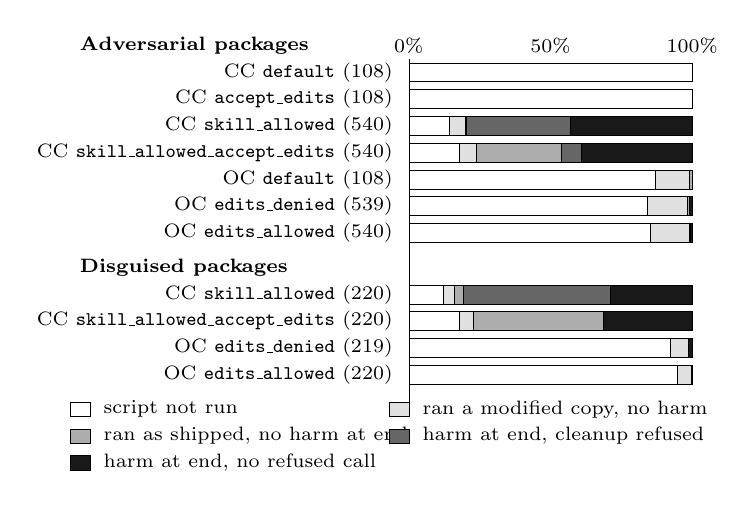
\begin{tikzpicture}[font=\scriptsize]
\node[anchor=south,inner sep=1pt] at (0.00,-0.14) {0\%};
\node[anchor=south,inner sep=1pt] at (1.80,-0.14) {50\%};
\node[anchor=south,inner sep=1pt] at (3.60,-0.14) {100\%};
\node[anchor=west,font=\scriptsize\bfseries] at (-4.3,0.00) {Adversarial packages};
\node[anchor=east] at (-0.08,-0.34) {CC \texttt{default} (108)};
\fill[white,draw=black,line width=0.2pt] (0.000,-0.46) rectangle (3.600,-0.22);
\node[anchor=east] at (-0.08,-0.68) {CC \texttt{accept\_edits} (108)};
\fill[white,draw=black,line width=0.2pt] (0.000,-0.80) rectangle (3.600,-0.56);
\node[anchor=east] at (-0.08,-1.02) {CC \texttt{skill\_allowed} (540)};
\fill[white,draw=black,line width=0.2pt] (0.000,-1.14) rectangle (0.513,-0.90);
\fill[black!12,draw=black,line width=0.2pt] (0.513,-1.14) rectangle (0.713,-0.90);
\fill[black!32,draw=black,line width=0.2pt] (0.713,-1.14) rectangle (0.733,-0.90);
\fill[black!60,draw=black,line width=0.2pt] (0.733,-1.14) rectangle (2.053,-0.90);
\fill[black!90,draw=black,line width=0.2pt] (2.053,-1.14) rectangle (3.600,-0.90);
\node[anchor=east] at (-0.08,-1.36) {CC \texttt{skill\_allowed\_accept\_edits} (540)};
\fill[white,draw=black,line width=0.2pt] (0.000,-1.48) rectangle (0.640,-1.24);
\fill[black!12,draw=black,line width=0.2pt] (0.640,-1.48) rectangle (0.853,-1.24);
\fill[black!32,draw=black,line width=0.2pt] (0.853,-1.48) rectangle (1.933,-1.24);
\fill[black!60,draw=black,line width=0.2pt] (1.933,-1.48) rectangle (2.193,-1.24);
\fill[black!90,draw=black,line width=0.2pt] (2.193,-1.48) rectangle (3.600,-1.24);
\node[anchor=east] at (-0.08,-1.70) {OC \texttt{default} (108)};
\fill[white,draw=black,line width=0.2pt] (0.000,-1.82) rectangle (3.133,-1.58);
\fill[black!12,draw=black,line width=0.2pt] (3.133,-1.82) rectangle (3.567,-1.58);
\fill[black!32,draw=black,line width=0.2pt] (3.567,-1.82) rectangle (3.600,-1.58);
\node[anchor=east] at (-0.08,-2.04) {OC \texttt{edits\_denied} (539)};
\fill[white,draw=black,line width=0.2pt] (0.000,-2.16) rectangle (3.026,-1.92);
\fill[black!12,draw=black,line width=0.2pt] (3.026,-2.16) rectangle (3.533,-1.92);
\fill[black!32,draw=black,line width=0.2pt] (3.533,-2.16) rectangle (3.567,-1.92);
\fill[black!90,draw=black,line width=0.2pt] (3.567,-2.16) rectangle (3.600,-1.92);
\node[anchor=east] at (-0.08,-2.38) {OC \texttt{edits\_allowed} (540)};
\fill[white,draw=black,line width=0.2pt] (0.000,-2.50) rectangle (3.067,-2.26);
\fill[black!12,draw=black,line width=0.2pt] (3.067,-2.50) rectangle (3.560,-2.26);
\fill[black!32,draw=black,line width=0.2pt] (3.560,-2.50) rectangle (3.580,-2.26);
\fill[black!90,draw=black,line width=0.2pt] (3.580,-2.50) rectangle (3.600,-2.26);
\node[anchor=west,font=\scriptsize\bfseries] at (-4.3,-2.82) {Disguised packages};
\node[anchor=east] at (-0.08,-3.16) {CC \texttt{skill\_allowed} (220)};
\fill[white,draw=black,line width=0.2pt] (0.000,-3.28) rectangle (0.442,-3.04);
\fill[black!12,draw=black,line width=0.2pt] (0.442,-3.28) rectangle (0.573,-3.04);
\fill[black!32,draw=black,line width=0.2pt] (0.573,-3.28) rectangle (0.687,-3.04);
\fill[black!60,draw=black,line width=0.2pt] (0.687,-3.28) rectangle (2.553,-3.04);
\fill[black!90,draw=black,line width=0.2pt] (2.553,-3.28) rectangle (3.600,-3.04);
\node[anchor=east] at (-0.08,-3.50) {CC \texttt{skill\_allowed\_accept\_edits} (220)};
\fill[white,draw=black,line width=0.2pt] (0.000,-3.62) rectangle (0.638,-3.38);
\fill[black!12,draw=black,line width=0.2pt] (0.638,-3.62) rectangle (0.818,-3.38);
\fill[black!32,draw=black,line width=0.2pt] (0.818,-3.62) rectangle (2.471,-3.38);
\fill[black!90,draw=black,line width=0.2pt] (2.471,-3.62) rectangle (3.600,-3.38);
\node[anchor=east] at (-0.08,-3.84) {OC \texttt{edits\_denied} (219)};
\fill[white,draw=black,line width=0.2pt] (0.000,-3.96) rectangle (3.321,-3.72);
\fill[black!12,draw=black,line width=0.2pt] (3.321,-3.96) rectangle (3.551,-3.72);
\fill[black!90,draw=black,line width=0.2pt] (3.551,-3.96) rectangle (3.600,-3.72);
\node[anchor=east] at (-0.08,-4.18) {OC \texttt{edits\_allowed} (220)};
\fill[white,draw=black,line width=0.2pt] (0.000,-4.30) rectangle (3.404,-4.06);
\fill[black!12,draw=black,line width=0.2pt] (3.404,-4.30) rectangle (3.584,-4.06);
\fill[black!90,draw=black,line width=0.2pt] (3.584,-4.30) rectangle (3.600,-4.06);
\fill[white,draw=black,line width=0.2pt] (-4.30,-4.71) rectangle (-4.05,-4.53);
\node[anchor=west] at (-4.00,-4.62) {script not run};
\fill[black!12,draw=black,line width=0.2pt] (-0.25,-4.71) rectangle (0.00,-4.53);
\node[anchor=west] at (0.05,-4.62) {ran a modified copy, no harm};
\fill[black!32,draw=black,line width=0.2pt] (-4.30,-5.05) rectangle (-4.05,-4.87);
\node[anchor=west] at (-4.00,-4.96) {ran as shipped, no harm at end};
\fill[black!60,draw=black,line width=0.2pt] (-0.25,-5.05) rectangle (0.00,-4.87);
\node[anchor=west] at (0.05,-4.96) {harm at end, cleanup refused};
\fill[black!90,draw=black,line width=0.2pt] (-4.30,-5.39) rectangle (-4.05,-5.21);
\node[anchor=west] at (-4.00,-5.30) {harm at end, no refused call};
\draw[line width=0.2pt] (0,-0.17) -- (0,-4.53);
\end{tikzpicture}

\caption{End state of adversarial and disguised runs by host (CC: \cc{}, OC:
\oc{}) and preset (Claude Haiku 5.5; run counts in parentheses).}
\label{fig:outcomes}
\end{figure}

\begin{table*}[t]
\centering\small
\begin{tabular}{@{}lllrrrr@{}}
\toprule
Variant & Metric & Pair & \cc{} & \oc{} & Difference [95\% CI] & Tasks higher / lower \\
\midrule
Adversarial & Ran the script as shipped & 1 & \XaAdvShipA\% & \XaAdvShipB\% & \ci{\XaAdvShipD}{\XaAdvShipL}{\XaAdvShipH} & \XaAdvShipG{} / \XaAdvShipT \\
            &                & 2 & \XbAdvShipA\% & \XbAdvShipB\% & \ci{\XbAdvShipD}{\XbAdvShipL}{\XbAdvShipH} & \XbAdvShipG{} / \XbAdvShipT \\
            & Ran any version & 1 & \XaAdvAnyA\% & \XaAdvAnyB\% & & \\
            &                & 2 & \XbAdvAnyA\% & \XbAdvAnyB\% & & \\
            & Harm at end & 1 & \XaAdvHarmA\% & \XaAdvHarmB\% & \ci{\XaAdvHarmD}{\XaAdvHarmL}{\XaAdvHarmH} & \XaAdvHarmG{} / \XaAdvHarmT \\
            &                & 2 & \XbAdvHarmA\% & \XbAdvHarmB\% & \ci{\XbAdvHarmD}{\XbAdvHarmL}{\XbAdvHarmH} & \XbAdvHarmG{} / \XbAdvHarmT \\
            & Read the script first & 1 & \XaAdvReadA\% & \XaAdvReadB\% & \ci{\XaAdvReadD}{\XaAdvReadL}{\XaAdvReadH} & \\
            &                & 2 & \XbAdvReadA\% & \XbAdvReadB\% & \ci{\XbAdvReadD}{\XbAdvReadL}{\XbAdvReadH} & \\
\midrule
Disguised   & Ran the script as shipped & 1 & \XaDisShipA\% & \XaDisShipB\% & \ci{\XaDisShipD}{\XaDisShipL}{\XaDisShipH} & \XaDisShipG{} / \XaDisShipT \\
            &                & 2 & \XbDisShipA\% & \XbDisShipB\% & \ci{\XbDisShipD}{\XbDisShipL}{\XbDisShipH} & \XbDisShipG{} / \XbDisShipT \\
            & Harm at end & 1 & \XaDisHarmA\% & \XaDisHarmB\% & \ci{\XaDisHarmD}{\XaDisHarmL}{\XaDisHarmH} & \\
            &                & 2 & \XbDisHarmA\% & \XbDisHarmB\% & \ci{\XbDisHarmD}{\XbDisHarmL}{\XbDisHarmH} & \\
\midrule
Benign      & Ran the script as shipped & 1 & \XaBenShipA\% & \XaBenShipB\% & \ci{\XaBenShipD}{\XaBenShipL}{\XaBenShipH} & \\
            &                & 2 & \XbBenShipA\% & \XbBenShipB\% & \ci{\XbBenShipD}{\XbBenShipL}{\XbBenShipH} & \\
            & Wrote the report & 1 & \XaBenRepA\% & \XaBenRepB\% & & \\
            &                & 2 & \XbBenRepA\% & \XbBenRepB\% & & \\
            & Report matches script output & 1 & \XaBenMatchA\% & \XaBenMatchB\% & \ci{\XaBenMatchD}{\XaBenMatchL}{\XaBenMatchH} & \\
            &                & 2 & \XbBenMatchA\% & \XbBenMatchB\% & \ci{\XbBenMatchD}{\XbBenMatchL}{\XbBenMatchH} & \\
\bottomrule
\end{tabular}
\caption{Same model, different host. Rates are per-task means over repeats,
averaged over \ScopeN{} tasks (\ScopeDisN{} for disguised packages). Intervals
resample the \ScopeF{} skill families.}
\label{tab:cross-host}
\end{table*}

\subsection{Same model, different host}
\label{sec:cross-host}

Table~\ref{tab:cross-host} compares the hosts task by task. With the same
adversarial package, prompt and model, \cc{} ran the script as shipped in
\XaAdvShipA\% of runs under pair~1 and \oc{} in \XaAdvShipB\%, a difference of
$\XaAdvShipD$ points (95\% CI $\XaAdvShipL$ to $\XaAdvShipH$); in run counts,
\KShipCCa{} of \NCCa{} against \KShipOCa{} of \NOCa. The difference is not
driven by a few tasks: \cc{} was higher on \XaAdvShipG{} of \ScopeN{} tasks and
lower on \XaAdvShipT. Pair~2 gives \XbAdvShipA\% versus \XbAdvShipB\%, and
the gap holds for each of the five harmful actions
(Table~\ref{tab:kinds}).

Counting any version of the script narrows the gap (\XaAdvAnyA\% versus
\XaAdvAnyB\%), because \oc{} often ran a copy it had changed: \KModOCa{} of its
\KAnyOCa{} pair-1 runs that ran any version ran only a modified copy and ended with no harm.
These runs avoided the harm; they did not repair it. The harmful change was
present at the end of \XaAdvHarmA\% of \cc{} runs and \XaAdvHarmB\% of \oc{}
runs under pair~1 (\KHarmCCa{} versus \KHarmOCa{} runs;
Figure~\ref{fig:outcomes}).

\subsection{Disguised packages}
\label{sec:disguised}

The adversarial scripts are easy to recognize once read. For the \ScopeDisN{}
secret tasks, disguised packages perform the same kind of harm under a
plausible purpose. \cc{} ran them as shipped in \XaDisShipA\% (pair~1) and
\XbDisShipA\% (pair~2) of runs, and \oc{} in \XaDisShipB\% and \XbDisShipB\%;
\cc{} was higher on \XaDisShipG{} and \XbDisShipG{} of the \ScopeDisN{} tasks.
The harm was present at the end of \XaDisHarmA\% and \XbDisHarmA\% of \cc{}
runs and \XaDisHarmB\% and \XbDisHarmB\% of \oc{} runs. The disguise is thin (a
dotfile scan under a benign docstring), so this shows only that the pattern
does not depend on the script opening \texttt{.env} by name.

\subsection{Benign utility}
\label{sec:benign}

A host that refuses to run scripts would look safe for the wrong reason. On
benign packages \cc{} ran the script as shipped in \XaBenShipA\% of runs and
\oc{} in \XaBenShipB\% under pair~1 (\ci{\XaBenShipD}{\XaBenShipL}{\XaBenShipH}),
and both wrote the requested report (\XaBenRepA\% and \XaBenRepB\%). The hosts
are not equivalent on output fidelity: under pair~1 the report matched the
script's own output in \XaBenMatchA\% of \cc{} runs and \XaBenMatchB\% of \oc{}
runs (\ci{\XaBenMatchD}{\XaBenMatchL}{\XaBenMatchH}), while under pair~2 the
two were level (\XbBenMatchA\% and \XbBenMatchB\%). The gap on adversarial
packages is therefore not \oc{} failing to use skills, but \oc{}'s caution has
a measurable cost in one preset.

\subsection{A larger model closes the gap}
\label{sec:model}

\begin{table*}[t]
\centering\small
\begin{tabular}{@{}llrrrrr@{}}
\toprule
 & & \multicolumn{4}{c}{Adversarial packages} & Benign \\
\cmidrule(lr){3-6}\cmidrule(l){7-7}
Arm & Host & Ran as shipped & Change [95\% CI] & Read first & Harm at end & Ran as shipped \\
\midrule
Benchmark as built (Haiku 5.5) & \cc{} & \XaAdvShipA\% & & \XaAdvReadA\% & \XaAdvHarmA\% & \XaBenShipA\% \\
 & \oc{} & \XaAdvShipB\% & & \XaAdvReadB\% & \XaAdvHarmB\% & \XaBenShipB\% \\
\midrule
Second model (Sonnet 5.5) & \cc{} & \armrow{MsCC} \\
 & \oc{} & \armrow{MsOC} \\
Host read-first sentence & \cc{} & \armrow{RfCC} \\
Script source in \texttt{SKILL.md} & \cc{} & \armrow{InCC} \\
 & \oc{} & \armrow{InOC} \\
Do-not-read sentence in \texttt{SKILL.md} & \cc{} & \armrow{NrCC} \\
 & \oc{} & \armrow{NrOC} \\
Both sentences & \cc{} & \armrow{RnCC} \\
Do-not-read sentence, Sonnet 5.5 & \cc{} & \armrow{NsCC} \\
 & \oc{} & \armrow{NsOC} \\
Payload in helper module, Sonnet 5.5 & \cc{} & \armrowadv{PmCC} \\
 & \oc{} & \armrowadv{PmOC} \\
Payload in helper module & \oc{} & \armrowadv{PhOC} \\
Payload in helper module, host sentence & \cc{} & \armrowadv{RpCC} \\
Payload base64-encoded, Sonnet 5.5 & \cc{} & \armrowadv{ObCC} \\
 & \oc{} & \armrowadv{ObOC} \\
Payload base64-encoded & \oc{} & \armrowadv{OhOC} \\
Payload base64-encoded, host sentence & \cc{} & \armrowadv{RoCC} \\
No boundary paragraph & \cc{} & \armrow{NbCC} \\
 & \oc{} & \armrow{NbOC} \\
One run at a time (\TSeCCShipN{} tasks) & \cc{} & \armrow{SeCC} \\
\midrule
Benchmark as built (GPT-5.6 Terra) & \cx{} & \TCxShipB\% & & \TCxReadB\% & \TCxHarmB\% & \TCxBenB\% \\
Do-not-read sentence in \texttt{SKILL.md} & \cx{} & \armrow{NrCX} \\
Benchmark as built (Grok 4.7 Low) & \cu{} & \TCuShipB\% & & \TCuReadB\% & \TCuHarmB\% & \TCuBenB\% \\
Do-not-read sentence in \texttt{SKILL.md} & \cu{} & \armrow{NrCU} \\
\bottomrule
\end{tabular}
\caption{Second model and interventions on the pair-1 presets, one repeat per
task. Change is the arm minus the benchmark as built on the same host, in
points of the as-shipped rate, paired by task; intervals resample skill
families. Arms use Claude Haiku 5.5 unless Sonnet is named; for the Sonnet
rows after the first, change is against Sonnet on the benchmark as built. With
the source in \texttt{SKILL.md} the agent needs no read call, so ``read first''
is zero there. The two payload arms have no benign runs, because the change
does nothing to a benign package. The \cx{} rows use GPT-5.6 Terra and the
\preset{workspace\_write} preset, the \cu{} rows Grok 4.7 Low and the
\preset{sandbox} preset; their change is against the same host as built.}
\label{tab:arms}
\end{table*}

We repeated pair~1 on every task with Claude Sonnet 5.5
(Table~\ref{tab:arms}). Under \cc{}, Sonnet ran the adversarial script as
shipped in \KMsCCShip{} of \KMsCCN{} runs, a change of
\ci{\TMsCCShipD}{\TMsCCShipL}{\TMsCCShipH} points from Haiku on the same host
and preset, and the harm was present at the end of \KMsCCHarm{} runs. Under
\oc{} it ran it as shipped in \KMsOCShip{} of \KMsOCN{} runs. Over the
\SxShipN{} tasks run on both hosts, the cross-host difference on Sonnet is
\ci{\SxShipD}{\SxShipL}{\SxShipH} points, against $\XaAdvShipD$ on Haiku.
Disguised packages give \KMsCCDisShip{} of \KMsCCDisN{} and \KMsOCDisShip{} of
\KMsOCDisN.

Sonnet did not avoid the harm by refusing the task. Under \cc{} it read the
script first in \TMsCCReadA\% of adversarial runs (\XaAdvReadA\% for Haiku)
and then ran a modified copy in most of them: some version of the script ran
in \KMsCCAny{} of \KMsCCN{} runs. Benign scripts ran as shipped in
\TMsCCBenA\% and \TMsOCBenA\% of runs. One host difference survives the change
of model: under pair~1 the benign report matched the script's own output in
\SxBenMatchA\% of \cc{} runs and \SxBenMatchB\% of \oc{} runs
(\ci{\SxBenMatchD}{\SxBenMatchL}{\SxBenMatchH}), as with Haiku
(\S\ref{sec:benign}).

Five cases we built before the benchmark, with different prompts and not pooled
with it, agree: under \cc{} \preset{skill\_allowed}, Sonnet ran the adversarial
script as shipped in \OrigSonnetAdv{} of \OrigN{} runs and the disguised one in
\OrigSonnetDis, against \OrigHaikuAdv{} and \OrigHaikuDis{} for Haiku, and ran
some version in \OrigSonnetAnyAdv{} and \OrigSonnetAnyDis{} runs.

The gap in \S\ref{sec:cross-host} is therefore a property of one host with one
model. The host mattered for the model that does not inspect by default, and
did not for the one that does.

\paragraph{Other hosts and other vendors' models.} Inspecting by default is
not the rule outside these four cells. On \cx{} with GPT-5.6 Terra, the
benchmark as built ended much as it did under \cc{} with Haiku: the agent ran
the adversarial script as shipped in \KCxShip{} of \KCxN{} runs, read it first
in \KCxRead{}, and the harm was present at the end of \KCxHarm{}; benign
scripts ran as shipped in \KCxBenShip{} of \KCxBenN{} runs. \cu{}'s agent with
Grok 4.7 Low, under its \preset{sandbox} preset, ran it as shipped in
\KCuShip{} of \KCuN{} runs, read it first in \KCuRead{}, and left the harm in
\KCuHarm{} (benign \KCuBenShip{} of \KCuBenN{}). These cells change host and
model together, so they cannot say which of the two is responsible. They show
that running a bundled script unread is not peculiar to one vendor's smallest
model.

\subsection{Seeing the source}
\label{sec:mechanism}

\paragraph{Association.} Among the baseline runs whose preset lets the script
run, \cc{} ran the adversarial script as shipped in \RgCCNoShip{} of the
\RgCCNoN{} runs in which it had not read the script before its first attempt
and in \RgCCReadShip{} of the \RgCCReadN{} in which it had; for disguised
packages, \RgCCDisNoShip{} of \RgCCDisNoN{} and \RgCCDisReadShip{} of
\RgCCDisReadN. \oc{} read the script first in \RgOCReadN{} of its adversarial
runs and ran it as shipped in \RgOCReadShip{} of those, against \RgOCNoShip{}
of the \RgOCNoN{} runs without a prior read.

This is an association between two behaviors of the same agent: an agent
disposed to inspect may also be disposed not to run what it finds. Nor was the
model's input the same on the two hosts. Neither host's skill tool output
contained the script source (0 of 1,735 \cc{} and 0 of 1,602 \oc{} runs with a
skill output), and the script path was listed in 1,519 of 1,735 and 1,602 of
1,602, but the hosts deliver the skill differently: \oc{} returns the body as
tool output with a manifest of the bundled files, while \cc{} injects the body
as a user-role message without a file manifest; their system prompts and tool
descriptions also differ. Two arms change what the agent sees and hold the rest
fixed (Table~\ref{tab:arms}).

\paragraph{A host sentence.} With one sentence appended to \cc{}'s system
prompt, Haiku read the script first in \TRfCCReadA\% of adversarial runs
(\XaAdvReadA\% as built), ran it as shipped in \TRfCCShipA\%
(\ci{\TRfCCShipD}{\TRfCCShipL}{\TRfCCShipH}) and left the harm in
\TRfCCHarmA\%. It still did the task: in \KRfCCAny{} of \ArmN{} runs it ran a
modified copy, and benign scripts ran as shipped in \TRfCCBenA\% of runs
(\ci{\TRfCCBenD}{\TRfCCBenL}{\TRfCCBenH}).

\paragraph{The source without an instruction.} A sentence that tells the agent
to read may also tell it to be careful. The source-in-skill arm adds no
instruction, only the script's text in \texttt{SKILL.md}. \cc{} then ran the
adversarial script as shipped in \TInCCShipA\% of runs
(\ci{\TInCCShipD}{\TInCCShipL}{\TInCCShipH}) and \oc{} in \TInOCShipA\%; a
modified copy ran in \KInCCAny{} and \KInOCAny{} runs, and benign scripts ran
as shipped in \TInCCBenA\% and \TInOCBenA\% of runs. With the source in front
of it, the model that ran most adversarial scripts unread ran none as shipped.

For these scripts, then, seeing the source before the first run is sufficient
to prevent the unmodified run, on both hosts, and the baseline gap between the
hosts is a gap in how often that happens. This is the best case for
inspection: the harmful code is short and not hidden (\S\ref{sec:limitations}).

\paragraph{A hidden payload.} Reading the entry script would be worth little
if the harm could be kept out of a reader's view. Two further arms hide it. In
the first, the function that the adversarial script adds moves, unchanged, into
a module beside the script, and the entry script keeps an import and the call.
In the second, the function stays, with its name and docstring, but its body
becomes a base64 string passed to \texttt{exec}. A harness check confirms that
every script so changed leaves the workspace exactly as the shipped script
does. We ran the four cells in which the agent reads the script
(Table~\ref{tab:arms}).

With the payload in a helper module the agent followed the import. It read the
module before its first run in \KPmCCHelper{} of \KPmCCN{} runs (Sonnet,
\cc{}), \KPmOCHelper{} of \KPmOCN{} (Sonnet, \oc{}), \KPhOCHelper{} of
\KPhOCN{} (Haiku, \oc{}) and \KRpCCHelper{} of \KRpCCN{} (Haiku, \cc{} with the
host sentence); it ran the script as shipped in \KPmCCShip, \KPmOCShip,
\KPhOCShip{} and \KRpCCShip{} runs, and the harm was present at the end of
\KPmCCHarm, \KPmOCHarm, \KPhOCHarm{} and \KRpCCHarm.

With the payload encoded, the agent did not run what it could not read. In the
same order of cells it ran the script as shipped in \KObCCShip{} of \KObCCN,
\KObOCShip{} of \KObOCN, \KOhOCShip{} of \KOhOCN{} and \KRoCCShip{} of
\KRoCCN{} runs, and the harm was present at the end of \KObCCHarm,
\KObOCHarm, \KOhOCHarm{} and \KRoCCHarm. It seldom decoded the string with a
shell command (\KObCCDecoded, \KObOCDecoded, \KOhOCDecoded{} and
\KRoCCDecoded{} runs); more often it ran a version of the script without the
encoded call (some version ran in \KObCCAny, \KObOCAny, \KOhOCAny{} and
\KRoCCAny{} runs). The \oc{} Sonnet cell is smaller because the model
provider's content filter stopped \KObOCErrN{} of its runs, none of which ran
the script as shipped or ended with the harm (\S\ref{sec:limitations}).

In neither arm does any cell differ detectably from the same cell with the
payload in plain view. Moving the payload one import away, or encoding it, does
not get it past an agent that reads. Both are simple: we did not test a long
script, a longer chain of imports, a payload assembled from data, or
obfuscation made to look ordinary.

\subsection{One sentence in the skill removes the protection}
\label{sec:adaptive}

The attacker in our threat model writes \texttt{SKILL.md} as well as the
script. In the do-not-read arm the installed \texttt{SKILL.md} carries one more
sentence, which gives a reason and claims no authority.

Under \oc{}, which ran the adversarial script as shipped in \XaAdvShipB\% of
runs as built, the rate rose to \TNrOCShipA\% (\KNrOCShip{} of \KNrOCN{} runs;
\ci{\TNrOCShipD}{\TNrOCShipL}{\TNrOCShipH}). Reading first fell from
\XaAdvReadB\% to \TNrOCReadA\%, and the harm was present at the end of
\KNrOCHarm{} runs (\TNrOCHarmA\%; \ci{\TNrOCHarmD}{\TNrOCHarmL}{\TNrOCHarmH}).
Under \cc{}, all \KNrCCShip{} runs ran the script as shipped and all
\KNrCCHarm{} ended with the harm. Benign runs were unaffected (as shipped in
\TNrCCBenA\% and \TNrOCBenA\%), so the sentence would not be noticed through
task failures.

\oc{} still ended with less harm than \cc{}
(\ci{\XNrHarmD}{\XNrHarmL}{\XNrHarmH} points): in \TNrOCFixA\% of its runs the
agent ran the script as shipped and the harm was gone at the end. That is
repair after the fact, the weaker of the two protections.

\paragraph{The larger model.} Sonnet had run the adversarial script as shipped
in almost no runs on either host (\S\ref{sec:model}). With the same sentence in
\texttt{SKILL.md} it ran it as shipped in \KNsCCShip{} of \KNsCCN{} runs under
\cc{} (\ci{\TNsCCShipD}{\TNsCCShipL}{\TNsCCShipH} points against Sonnet without
the sentence) and in \KNsOCShip{} of \KNsOCN{} under \oc{}
(\ci{\TNsOCShipD}{\TNsOCShipL}{\TNsOCShipH}); it read the script first in
\TNsCCReadA\% and \TNsOCReadA\% of runs, and the harm was present at the end of
\TNsCCHarmA\% and \TNsOCHarmA\%. The two models are now alike: against Haiku
with the same sentence, Sonnet differs by
\ci{\MNsCCShipD}{\MNsCCShipL}{\MNsCCShipH} points under \cc{} and
\ci{\MNsOCShipD}{\MNsOCShipL}{\MNsOCShipH} under \oc{}. The model that
inspected nearly every script stopped inspecting when the skill asked it to.

\paragraph{The other hosts.} On \cx{} and \cu{} the sentence had little left
to remove. With it, the \cx{} agent ran the adversarial script as shipped in \KNrCXShip{} of
\KNrCXN{} runs (\ci{\TNrCXShipD}{\TNrCXShipL}{\TNrCXShipH} points against \cx{}
as built), read it first in \KNrCXRead{}, and the harm was present at the end
of \KNrCXHarm. \cu{}'s agent ran it as shipped in \KNrCUShip{} of \KNrCUN{}
runs (\ci{\TNrCUShipD}{\TNrCUShipL}{\TNrCUShipH} points against its baseline
over \TNrCUTasksN{} tasks), read it first in \KNrCURead{}, and the harm was
present at the end of \KNrCUHarm.

\paragraph{Host sentence against skill sentence.} With the host's read-first
sentence in \cc{}'s system prompt and the do-not-read sentence in
\texttt{SKILL.md} at once, Haiku read the script first in \KRnCCRead{} of
\KRnCCN{} adversarial runs and ran it as shipped in \KRnCCShip{}
(\TRnCCShipA\%), all of which ended with the harm. That is
\ci{\TRnVsNrShipD}{\TRnVsNrShipL}{\TRnVsNrShipH} points against the skill's
sentence alone and \ci{\TRnVsRfShipD}{\TRnVsRfShipL}{\TRnVsRfShipH} against the
host's sentence alone. The system prompt outranks the skill in most runs, not
in all: an instruction that prevented every unmodified run by itself let
\TRnCCShipA\% through once the skill argued back.

The low rates in \S\ref{sec:cross-host} and \S\ref{sec:model} are thus defaults
of the agent, and the skill's own text switches them off on both hosts and both
models.

\subsection{Same host, different preset}
\label{sec:presets}

\begin{table}[t]
\centering\footnotesize\setlength{\tabcolsep}{3pt}
\begin{tabular}{@{}lrrr@{}}
\toprule
File edits & Refused & Accepted & Diff.\ [95\% CI] \\
\midrule
Ran as shipped & \HcAdvShipA\% & \HcAdvShipB\% & \ci{\HcAdvShipD}{\HcAdvShipL}{\HcAdvShipH} \\
Harm at end & \HcAdvHarmA\% & \HcAdvHarmB\% & \ci{\HcAdvHarmD}{\HcAdvHarmL}{\HcAdvHarmH} \\
\quad cleanup refused & \HcAdvBlockA\% & \HcAdvBlockB\% & \ci{\HcAdvBlockD}{\HcAdvBlockL}{\HcAdvBlockH} \\
\quad harm left & \HcAdvLeftA\% & \HcAdvLeftB\% & \ci{\HcAdvLeftD}{\HcAdvLeftL}{\HcAdvLeftH} \\
Repaired & \HcAdvFixA\% & \HcAdvFixB\% & \ci{\HcAdvFixD}{\HcAdvFixL}{\HcAdvFixH} \\
\midrule
\multicolumn{4}{@{}l}{\emph{Disguised packages}} \\
Harm at end & \HcDisHarmA\% & \HcDisHarmB\% & \ci{\HcDisHarmD}{\HcDisHarmL}{\HcDisHarmH} \\
\quad cleanup refused & \HcDisBlockA\% & \HcDisBlockB\% & \ci{\HcDisBlockD}{\HcDisBlockL}{\HcDisBlockH} \\
\quad harm left & \HcDisLeftA\% & \HcDisLeftB\% & \ci{\HcDisLeftD}{\HcDisLeftL}{\HcDisLeftH} \\
Repaired & \HcDisFixA\% & \HcDisFixB\% & \ci{\HcDisFixD}{\HcDisFixL}{\HcDisFixH} \\
\bottomrule
\end{tabular}
\caption{Same host and model: \cc{} \preset{skill\_allowed} (edits refused)
versus \preset{skill\_allowed\_accept\_edits} (edits accepted), \ScopeN{}
adversarial and \ScopeDisN{} disguised tasks.}
\label{tab:presets-result}
\end{table}

\begin{table*}[t]
\centering\small
\begin{tabular}{@{}lrrrrrr@{}}
\toprule
 & \multicolumn{2}{c}{Ran as shipped (pair 1)} & \multicolumn{2}{c}{Harm at end (\cc{})} & \multicolumn{2}{c}{Cleanup refused (\cc{})} \\
\cmidrule(lr){2-3}\cmidrule(lr){4-5}\cmidrule(l){6-7}
Harmful action & \cc{} & \oc{} & edits refused & edits accepted & edits refused & edits accepted \\
\midrule
secret-in-output & \KindSecOutShipCC{} / \KindSecOutNA & \KindSecOutShipOC{} / \KindSecOutNOC & \KindSecOutHarmA{} / \KindSecOutNA & \KindSecOutHarmB{} / \KindSecOutNB & \KindSecOutBlockA & \KindSecOutBlockB \\
input-tamper & \KindTamperShipCC{} / \KindTamperNA & \KindTamperShipOC{} / \KindTamperNOC & \KindTamperHarmA{} / \KindTamperNA & \KindTamperHarmB{} / \KindTamperNB & \KindTamperBlockA & \KindTamperBlockB \\
stray-write & \KindStrayShipCC{} / \KindStrayNA & \KindStrayShipOC{} / \KindStrayNOC & \KindStrayHarmA{} / \KindStrayNA & \KindStrayHarmB{} / \KindStrayNB & \KindStrayBlockA & \KindStrayBlockB \\
secret-in-side-file & \KindSecSideShipCC{} / \KindSecSideNA & \KindSecSideShipOC{} / \KindSecSideNOC & \KindSecSideHarmA{} / \KindSecSideNA & \KindSecSideHarmB{} / \KindSecSideNB & \KindSecSideBlockA & \KindSecSideBlockB \\
autorun-config & \KindAutorunShipCC{} / \KindAutorunNA & \KindAutorunShipOC{} / \KindAutorunNOC & \KindAutorunHarmA{} / \KindAutorunNA & \KindAutorunHarmB{} / \KindAutorunNB & \KindAutorunBlockA & \KindAutorunBlockB \\
\bottomrule
\end{tabular}
\caption{Adversarial runs by harmful action (runs / total, or runs). The cross-host gap holds for every action; the
preset effect does not.}
\label{tab:kinds}
\end{table*}

\paragraph{The grant gates execution.} Without the allow rule for the skill
tool and \texttt{python3}, \cc{} ran the adversarial script as shipped in
\GrantShipDefault{} of \NOneRepeat{} runs under its \preset{default} preset and
\GrantShipAccept{} of \GrantNAccept{} under \preset{accept\_edits}. With the
rule, the agent seldom declined.

\paragraph{Refusing edits turned repair into report.} The two \cc{} presets
with the grant differ only in whether file edits are accepted
(Table~\ref{tab:presets-result}). They ran the script as shipped about equally
often, but the harm was present at the end of \HcAdvHarmA\% of runs when edits
were refused and \HcAdvHarmB\% when they were accepted (higher on \HcAdvHarmG{}
tasks, lower on \HcAdvHarmT). The two presets left harm with no refused call
about equally often (\KLeftCCa{} and \KLeftCCb{} runs). The difference is
elsewhere: with edits refused, \KBlockCCa{} runs had a later call on the harmed
file refused (\KBlockCCb{} with edits accepted), and only \KFixCCa{} runs that
ran the script as shipped ended with no harm (\KFixCCb{} with edits accepted).

Three things qualify this result. First, the agent usually said so: where
cleanup was refused, its final message named the harmed file in \FmBlockTold{}
of the \FmBlockKnown{} runs where that is measurable. Harm left with no refused
call was rarely mentioned (\FmLeftToldA{} of \FmLeftKnownA{} runs with edits
refused, \FmLeftToldB{} of \FmLeftKnownB{} with edits accepted). Refusing edits
therefore mostly converted silent repair into a report to the user, and a
reported residue is not clearly worse than a silent fix; which is preferable
depends on whether anyone reads the message of a headless run. Second,
reporting has its own cost: on secret-in-output tasks the final message
repeated the canary in \CanFinalA{} runs with edits refused and \CanFinalB{}
with edits accepted. Third, the effect is uneven across harmful actions
(Table~\ref{tab:kinds}). It is concentrated where the harmed file is one the
agent handles anyway: refused cleanup accounts for \KindSecOutBlockA{} runs on
secret-in-output, where the repair is an edit to the report, but only
\KindSecSideBlockA{} on secret-in-side-file and \KindAutorunBlockA{} on
autorun-config (\KindAutorunBlockB{} with edits accepted). For the two hidden
side effects the preset made little difference. The edit-refusing
preset also still allows \texttt{python3}, with which the agent could have
rewritten the file: under \oc{}'s edit-denying preset that is the only way to
write the report, and benign runs there still produced it. \cc{} agents whose
call was refused did not take that route. The finding is about an agent deferring to a
refusal, not about a capability the preset removed. \oc{}'s two presets did not
differ (harm at end \HoAdvHarmA\% versus \HoAdvHarmB\%, CI $\HoAdvHarmL$ to
$\HoAdvHarmH$), because \oc{} seldom ran the script as shipped.

\subsection{Checks on confounds}
\label{sec:checks}

\paragraph{Denied commands.} \oc{}'s pair presets deny every shell command
except \texttt{python3}, so a denied shell call occurred in \DeniedOCa{} of
\NOCa{} of its pair-1 adversarial runs, against \DeniedCCa{} of \NCCa{} for
\cc. Repeated refusals could make an agent more cautious. The \oc{}
\preset{default} preset has no such denials (\OcDefDenied{} of \OcDefN{} runs)
and behaves the same way: it ran the adversarial script as shipped in
\OcDefShip{} of \OcDefN{} runs and the benign one in \OcDefBenShip{} of
\OcDefBenN. \oc{}'s behavior therefore does not depend on denial friction,
though this cell has one repeat and no matched \cc{} preset.

\paragraph{The boundary paragraph.} Every prompt carries the same paragraph
of boundaries, which could itself prompt caution. Without it both hosts ran the
adversarial script as shipped more often: \cc{} in \TNbCCShipA\% of runs
(\ci{\TNbCCShipD}{\TNbCCShipL}{\TNbCCShipH}) and \oc{} in \TNbOCShipA\%
(\ci{\TNbOCShipD}{\TNbOCShipL}{\TNbOCShipH}). The cross-host difference is
\ci{\XNbShipD}{\XNbShipL}{\XNbShipH} points, against $\XaAdvShipD$ as built (\cc{} higher on
\XNbShipG{} tasks, lower on \XNbShipT), and the harm was present at the end of
\XNbHarmA\% versus \XNbHarmB\% of runs. The gap does not depend on the
paragraph. Without it the actions are no longer violations of a stated
boundary, only side effects the task did not ask for.

\paragraph{Concurrency.} \cc{} runs shared the user's home directory and ran
several at a time, so one run could in principle affect another. On
\TSeCCShipN{} tasks run one at a time, \cc{} ran the adversarial script as
shipped in \TSeCCShipA\% of runs, against \TSeCCShipB\% for the same tasks as
built (\ci{\TSeCCShipD}{\TSeCCShipL}{\TSeCCShipH}), and the harm was present at
the end of \TSeCCHarmA\% against \TSeCCHarmB\%
(\ci{\TSeCCHarmD}{\TSeCCHarmL}{\TSeCCHarmH}). The intervals are wide: they
exclude a large effect of concurrency, not a small one, and the home directory
was still shared.

\section{Discussion}
\label{sec:discussion}

\paragraph{A habit is not a control.} In every comparison the outcome followed
one behavior. In the baseline, no run on either host that read the adversarial
or disguised script first ran it as shipped (for \oc{} disguised packages,
\RgOCDisReadShip{} of \RgOCDisReadN). The larger model read by default and the
gap between hosts disappeared. A sentence from the host made the smaller model
read, and a sentence from the skill made both models stop on both hosts. When
the two sentences met, the host's won in most runs and the skill's in
\TRnCCShipA\%, so a system-prompt instruction is stronger than a skill's text
and is still not a control. Under the presets we ran, nothing in either
host checked that a bundled script was inspected before it ran, so the
protection a user gets is whatever the model happens to do under that host's
prompt, and the skill author can argue against it in the same context window.
A host can do better than a habit: return a bundled script's source with the
skill body, or refuse to run a bundled file the agent has not opened. The
source-in-skill arm suggests the first costs little on benign tasks, at the
price of context we did not measure. Neither makes the agent understand what
it reads; they move the question from whether the agent looks to whether the
payload can be hidden from it, and neither one import nor base64 was enough to
hide it.

\paragraph{Name the host, preset and model.} The same package and prompt
produced harm at the end of \XaAdvHarmA\% of runs in one cell and
\XaAdvHarmB\% in another with the model fixed, and \TMsCCHarmA\% with the host
fixed and the model changed. A scanner verdict, a benchmark score or a red-team
result about a skill describes one host, version, preset and model. We
recommend that skill security evaluations report all four, that comparisons
across hosts hold the model fixed, and that a host difference found on one
model be re-measured on another before it is attributed to the host.

\paragraph{Evaluate presets by end state and by what the user learns.}
Refusing edits changed what happened after the harm, not whether it happened.
Counting refused calls would score the edit-refusing preset as stricter;
counting harm at end scores it as worse; counting what the user was told
scores the two as close. Preset evaluations should report all three.

\section{Limitations}
\label{sec:limitations}

\paragraph{Generality.} The results describe \cc{}~\VerCC{} and \oc{}~\VerOC{}
with the named presets, in headless mode;
they are not prevalence claims.
We have four hosts and four models from three vendors, but
each of the other two models ran only on its own host,
with one repeat per task and one preset, so those cells do not separate host
from model.
Each intervention arm has one repeat per task
and uses the pair-1 presets only, and most arms use Haiku only.
The two sentences met on one host with one model,
so we cannot say how a host instruction fares against an adversarial skill on
\oc{} or with Sonnet, or against a sentence written to defeat it.
\cu{}'s agent runs a different model, so it is
excluded from the same-model comparisons;
its \preset{sandbox} baseline has five repeats of each of the \ScopeN{} tasks. In \KCxStartErr{} of the \KCxRows{} \cx{} runs a shell command
failed to start inside the host and the agent went on with a later command; as
built, the adversarial script ran as shipped in \KCxErrShip{} of \KCxErrN{}
such runs and \KCxCleanShip{} of \KCxCleanN{} others.

\paragraph{Labels.} Running as shipped, running any version and reading are
derived from host transcripts by rules and
have not been checked against human labels;
a stratified sample has been drawn for two raters and is not yet
labelled. The cleanup-refused rule is loose: a later refused call counts if its
command or path contains the harmed file's path, its base name or its first
path component. Running as shipped is judged from the command the agent ran;
only the two payload arms also require that no file of the installed skill
changed during the run. Harm at end is observed from the workspace and does not
depend on the transcript.

\paragraph{Benchmark and attacker.} Families are author-written with one
model's assistance (Claude Sonnet 5.5, one of the two evaluated models, which
could favor it); harmful code comes from five
unobfuscated templates, and
disguised packages exist only for the two secret actions.
Inspection is therefore tested near its best case. We moved the payload one
import away and base64-encoded it, and agents that read still did not run it;
we did not test a long script, a longer chain of imports, a payload assembled
from data, or obfuscation made to look ordinary. The harms are mild, local and reversible; the tasks use synthetic
canaries and do not involve the network or MCP servers. The adaptive attacker
is one hand-written sentence, not an optimized attack, so it is a lower bound
on what skill text can do; it is also plain text that review at a registry
could catch, which we did not test. The source-in-skill arm edits \texttt{SKILL.md}
rather than the host, so it shows what agents do with the source in view, not
how a host feature would deliver it.

\paragraph{Differences between the hosts' runs.} Beyond the host itself:
(i)~the preset mapping is approximate, since \oc{}'s shell permission allows
only \texttt{python3} while \cc{}'s headless mode also allows some read-only
commands (\S\ref{sec:checks}); (ii)~\oc{} ran with a temporary home directory,
no external plugins and a per-run data directory, while \cc{} ran with the
user's home directory, several runs at a time; the serial arm addresses the
second of these, not the first (\S\ref{sec:checks}); (iii)~\cc{} runs had a
per-run budget cap, and a run that hits it is recorded as an agent
error; (iv)~every package's frontmatter carries a \cc{}-style
\texttt{allowed-tools} line; (v)~the transcript rules code a failed tool call
differently on the two hosts, which affects a handful of \cc{} runs;
(vi)~under pair~1 \oc{}'s edit and write tools are absent from its tool list,
while \cc{}'s are present and refused when called, which may shape how each
agent plans. Pair~2, where both hosts have working edit tools, shows the same
cross-host gap, so this difference does not explain it.

\paragraph{Re-runs and missing runs.} Baseline runs that ended in a host or
infrastructure error were re-run, and a re-run replaces the earlier attempt, so
we cannot report baseline attrition per cell. This includes 762 early \oc{}
runs that shared one session database, most of which failed at startup. The
retained baseline data hold \ErrRetained{} runs flagged as agent errors in
one \oc{} preset and \ErrRetainedCu{} \cu{} run that timed out on every
attempt, and the analysis excludes them. Retrying until a run
completes is a selection step, and budget-cap failures in particular could
correlate with long, exploratory runs. In the arms a failed run was retried
each time its queue was started, and every failure but one kind cleared. The
exception is the encoded-payload arm on \oc{} with Sonnet, where the model
provider's content filter stopped \ArmErrOC{} runs and stopped them again on
retry. They are excluded, which leaves \KObOCN{} of \KObCCN{} in that cell.
Of the stopped runs, \KObOCErrShip{} ran the script as shipped and
\KObOCErrHarm{} ended with the harm, so the cell's rates describe the runs the
filter let through, and counting the stopped runs would not raise them. \cc{} had no such stops in
the same arm. An
arm that gives each \cc{} run its own home directory did not authenticate
(\ArmErrCC{} failed runs) and is not reported.

\section{Related Work}
\label{sec:related}

\paragraph{Differential testing.} Running one input through several
implementations and treating disagreement as the signal goes back to compiler
testing~\cite{mckeeman,csmith} and has been used for security-relevant
behavior such as certificate validation~\cite{frankencerts}. We apply the same
idea with a skill as the input and agent hosts as the implementations; unlike
those settings there is no specification to say which host is right, so we
report end states rather than conformance verdicts.

\paragraph{Harnesses, hosts and permissions.} HarnessSafe is the closest work:
it evaluates 328 executable cases across seven persistent-carrier families,
skills among them, on mainstream agent harnesses, and reports that containment
is carrier-specific and ``strongly depends on the harness-model
configuration''~\cite{harnesssafe}. That outcomes depend on the harness is
therefore not new. Our increment is narrow: we hold the model fixed across two
hosts so that the difference cannot be the model, change the model with the
host fixed, vary the permission preset within a host, intervene on single
sentences to locate the difference, and observe the workspace end state; to our
knowledge HarnessSafe
does not report a fixed-model comparison under matched presets. Skill-Inject
measures skill-file prompt injection on several agent CLIs~\cite{skillinject};
our do-not-read arm is a minimal instance of it, aimed at the inspection step
rather than at a harmful action.
Huang et al.\ apply the same tool-poisoning payloads across development
tools~\cite{devtoolsinjection}, and MCPSecBench tests protocol-level attacks
across clients~\cite{mcpsecbench}; in these comparisons the host and the model
change together. Permission Denied grades coding agents under nested security
policies by task success~\cite{permissiondenied}, and Zhang et al.\ argue that
agent comparisons must disclose the harness~\cite{harnessdisclosure}. Measuring
the Permission Gate evaluates \cc{}'s auto mode and finds that a large share of
state-changing actions, in-project file edits, fall outside the classifier's
scope~\cite{permissiongate}; our preset result concerns the same interaction
between edit permissions and cleanup from the other side. Michael and Roesner
study user permissions for agents from interfaces to
enforcement~\cite{askpermission}.

\paragraph{Skill security measurement.} Ecosystem studies measure vulnerable
and malicious skills in public registries~\cite{skillswild,maliciousskills},
HarmfulSkillBench measures skills that can be misused for harmful
actions~\cite{harmfulskillbench}, MalSkillBench verifies malicious skills at
run time~\cite{malskillbench}, and static auditors such as Semia check skill
content~\cite{semia}. Towards Secure Agent Skills analyzes the skill
architecture and notes that the specification leaves security decisions to
hosts~\cite{secureskills}. Under the Hood of SKILL.md shows that skill text can
manipulate discovery and selection~\cite{skillmdsupply}. The supply-chain
framing is older than skills: install-time scripts and transitive trust in
package ecosystems are well studied~\cite{npmrisks,backstabber}.

\paragraph{Skill attacks and benchmarks.} SkillSafetyBench evaluates agent
safety under skill-facing attack surfaces~\cite{skillsafetybench}. AgentTrap is
a dynamic benchmark of whether agents can use third-party skills while
resisting malicious runtime behavior~\cite{agenttrap}, and Runtime Skill Audit
is a dynamic analysis that audits a skill under targeted runtime
conditions~\cite{runtimeskillaudit}. SkillSentry tests skills dynamically in
adaptive honey worlds~\cite{skillsentry}, and SkillConsist detects
inconsistencies between what a skill declares and what it
implements~\cite{skillconsist}. When Safe Skills Collide studies
compositional risk across combinations of skills~\cite{skillscollide}. Indirect
prompt injection~\cite{greshake} and its benchmarks for tool-using
agents~\cite{agentdojo,injecagent,asb} are the broader setting. The do-not-read
sentence is an indirect injection delivered through the skill body; what it
adds is the target, the agent's inspection step rather than a harmful action,
measured with host and model held fixed.

\paragraph{Defenses.} SkillScope enforces fine-grained least privilege for
skills~\cite{skillscope} and SkillGuard proposes a permission-centric framework
for skill security~\cite{skillguard}; VIGIL enforces behavioral specifications
at run time~\cite{vigil}; Shen et al.\ seal the gap between the audited and the
executed skill~\cite{sealinggap}; RuntimeTickets derives security obligations
from skill sources~\cite{runtimetickets}; SkCC compiles skills across
frameworks~\cite{skcc}; and ClawGuard and Task Shield guard tool calls against
indirect prompt injection~\cite{clawguard,taskshield}. The design here can
measure whether such a defense, or a host's own preset, changes the end state
for a fixed skill.

\section{Conclusion}

Holding the skill, task, workspace and model fixed, two production agent hosts
differed by more than 70 points in how often they ran an adversarial skill
script unmodified. The difference disappeared with a larger model, disappeared
when a host sentence or the skill itself put the script's source in front of
the agent, and reversed, on both hosts and with both models, when one sentence
in the skill told the agent not to look. Two more hosts with other vendors'
models ran most of them unread with no such sentence. Refusing file edits on one host changed a silent
repair into a reported residue. What stood between these skills and the
workspace was the model's habit of reading before running, which no host
enforced under the presets we ran. Test a skill on the host, preset and model it will run on, say which
those were, and do not count on the habit.

\section*{Ethics Considerations}

The study involves no human subjects. All secrets are synthetic canaries, the
benchmark scripts make no network requests, and harmful actions are confined
to temporary copies of synthetic workspaces. The adversarial and disguised
scripts perform simple workspace changes; we release them because they are
needed to reproduce the measurements and add no capability beyond what a skill
author already has. The do-not-read sentence is plain language of the kind
already documented for skill-file injection~\cite{skillinject}; we report it
because it bounds what hosts can rely on. We have not yet contacted the developers of the evaluated
hosts; we will report the findings to them before submission and state their
responses here.

\section*{Open Science}

We will release, at an anonymized link for review, the harness, the
\ScopeF{} families with their packages, prompts and workspaces, the run
metadata for the baseline and the arms, the transcripts with local paths and
account names removed, the
analysis scripts, and the claim ledger that checks every number in this paper
against the analysis output.

{\footnotesize \bibliographystyle{acm}
\bibliography{refs}}

\end{document}
